%!TEX root=../../main.tex

\chapter{Inference for numerical data}
\label{inferenceForNumericalData}


Chapter~\ref{foundationsForInference} introduced some primary tools of statistical inference\textemdash point estimates, interval estimates, and hypothesis tests. This chapter examines settings where these tools are often used, including the analysis of paired observations and the comparison of two or more independent groups. The chapter also covers the important topic of estimating a sample size when a study is being designed.  The chapter starts with introducing a new distribution, the $t$-distribution, which can be used for small sample sizes. 


%__________________
\section{Inference for one-sample means with the $t$-distribution}
\label{oneSampleMeansWithTDistribution}

The tools studied in Chapter~\ref{foundationsForInference} all made use of the $t$-statistic from a sample mean,
\[t = \frac{\overline{x} - \mu}{s},\]
where the parameter $\mu$ is a population mean, and $\overline{x}$ and $s$ are the sample mean and standard deviation. Tests and confidence intervals were restricted to samples of at least 30 independent observations from a population where there was no evidence of strong skewness. This allowed for the Central Limit Theorem to be applied, justifying use of the normal distribution to calculate probabilities for the $t$-statistic. 

In sample sizes smaller than 30, if the data are approximately symmetric and there are no large outliers, the $t$-statistic has what is called a $t$-distribution. When the normal distribution is used as the sampling distribution of the $t$-statistic, $s$ is essentially being treated as a good replacement for the unknown population standard deviation $\sigma$. However, the sample standard deviation $s$, as an estimate of $\sigma$, has its own inherent variability like $\overline{x}$. The $t$ density function adjusts for the variability in $s$ by having more probability in the left and right tails than the normal distribution.

\subsection{The $t$-distribution}
\label{introducingTheTDistribution}

\index{t-distribution|(}
\index{distribution!$t$|(}

Figure~\ref{tDistCompareToNormalDist} shows a $t$ and normal distributions. Like the standard normal distribution, the $t$-distribution is unimodal and symmetric about zero.  But the tails of a $t$-distribution are thicker than for the normal, so observations are more likely to fall beyond two standard deviations from the mean than under the normal distribution.\footnote{The standard deviation of the $t$-distribution is actually a little more than 1. However, it is useful to always think of the $t$-distribution as having a standard deviation of 1 in all of our applications.} While the estimate of the standard error will be less accurate with smaller sample sizes, the thick tails of the $t$-distribution correct for the variability in $s$.

\begin{figure}
\centering
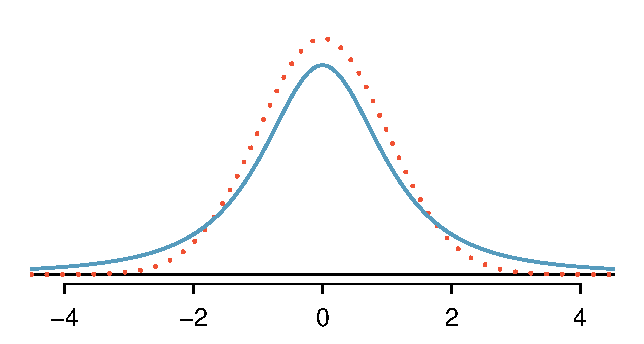
\includegraphics[height=45mm]{ch_inference_for_means_oi_biostat/figures/tDistCompareToNormalDist/tDistCompareToNormalDist}
\caption{Comparison of a $t$-distribution (solid line) and a normal distribution (dotted line).}
\label{tDistCompareToNormalDist}
\end{figure}

The $t$-distribution can be described as a family of symmetric distributions with a single parameter: degrees of freedom, which equals $n$ - 1. Several $t$-distributions are shown in Figure~\ref{tDistConvergeToNormalDist}. When there are more degrees of freedom, the $t$-distribution looks very much like the standard normal distribution. With degrees of freedom of 30 or more, the $t$-distribution is nearly indistinguishable from the normal distribution. Since the $t$-statistics in Chapter~\ref{foundationsForInference} were associated with sample sizes of at least 30, the degrees of freedom for the corresponding $t$-distributions were large enough to justify use of the normal distribution to calculate probabilities. 

\begin{figure}
\centering
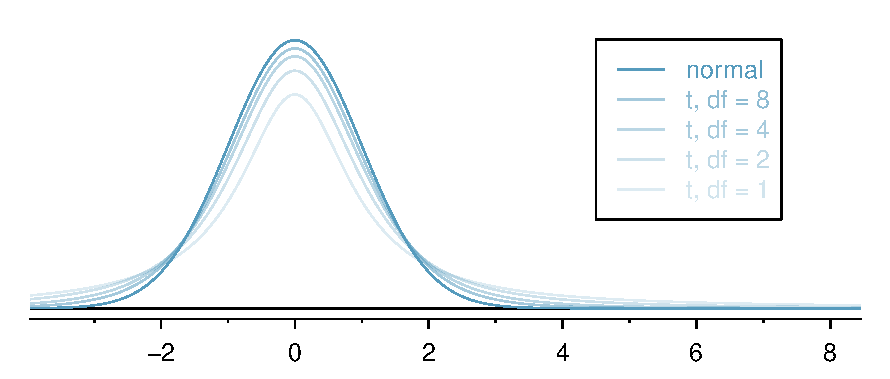
\includegraphics[width=0.8\textwidth]{ch_inference_for_means_oi_biostat/figures/tDistConvergeToNormalDist/tDistConvergeToNormalDist}
\caption{The larger the degrees of freedom, the more closely the $t$-distribution resembles the standard normal model.}
\label{tDistConvergeToNormalDist}
\end{figure}

\begin{termBox}{\tBoxTitle{Degrees of freedom (df)}
The degrees of freedom characterize the shape of the $t$-distribution. The larger the degrees of freedom, the more closely the distribution approximates the normal model.}
\end{termBox}

Probabilities for the $t$-distribution can be calculated either by using distribution tables or using statistical software. The use of software has become the preferred method because it is more accurate, allows for complete flexibility in the choice of $t$-values on the horizontal axis, and is not limited to a small range of degrees of freedom. This remainder of this section illustrates the use of a \term{t-table}, partially shown in Table~\ref{tTableSample}, in place of the normal probability table. A larger $t$-table is in Appendix~\ref{tDistributionTable} on page~\pageref{tDistributionTable}.  The \textsl{R Companion} illustrates the use of the \textsl{R} functions \texttt{pt} and \texttt{qt} to calculate probabilities for the $t$-distribution.  Readers intending to use software can skip to the next section.


\begin{table}[hht]
\centering
\begin{tabular}{r | rrr rr}
one tail & \hspace{1.5mm}  0.100 & \hspace{1.5mm} 0.050 & \hspace{1.5mm} 0.025 & \hspace{1.5mm} 0.010 & \hspace{1.5mm} 0.005  \\
two tails & 0.200 & 0.100 & 0.050 & 0.020 & 0.010 \\
\hline
{$df$} \hfill 1  &  {\normalsize  3.08} & {\normalsize  6.31} & {\normalsize 12.71} & {\normalsize 31.82} & {\normalsize 63.66}  \\ 
2  &  {\normalsize  1.89} & {\normalsize  2.92} & {\normalsize  4.30} & {\normalsize  6.96} & {\normalsize  9.92}  \\ 
3  &  {\normalsize  1.64} & {\normalsize  2.35} & {\normalsize  3.18} & {\normalsize  4.54} & {\normalsize  5.84}  \\ 
$\vdots$ & $\vdots$ &$\vdots$ &$\vdots$ &$\vdots$ & \\
17  &  {\normalsize  1.33} & {\normalsize  1.74} & {\normalsize  2.11} & {\normalsize  2.57} & {\normalsize  2.90}  \\ 
\highlightO{18}  &  \highlightO{\normalsize  1.33} & \highlightO{\normalsize  1.73} & \highlightO{\normalsize  2.10} & \highlightO{\normalsize  2.55} & \highlightO{\normalsize  2.88}  \\ 
19  &  {\normalsize  1.33} & {\normalsize  1.73} & {\normalsize  2.09} & {\normalsize  2.54} & {\normalsize  2.86}  \\ 
20  &  {\normalsize  1.33} & {\normalsize  1.72} & {\normalsize  2.09} & {\normalsize  2.53} & {\normalsize  2.85}  \\ 
$\vdots$ & $\vdots$ &$\vdots$ &$\vdots$ &$\vdots$ & \\
400  &  {\normalsize  1.28} & {\normalsize  1.65} & {\normalsize  1.97} & {\normalsize  2.34} & {\normalsize  2.59}  \\ 
500  &  {\normalsize  1.28} & {\normalsize  1.65} & {\normalsize  1.96} & {\normalsize  2.33} & {\normalsize  2.59}  \\ 
$\infty$  &  {\normalsize  1.28} & {\normalsize  1.64} & {\normalsize  1.96} & {\normalsize  2.33} & {\normalsize  2.58}  \\ 
\end{tabular}
\caption{An abbreviated look at the $t$-table. Each row represents a different $t$-distribution. The columns describe the cutoffs for specific tail areas. The row with $df=18$ has been \highlightO{highlighted}.}
\label{tTableSample}
\end{table}

Each row in the $t$-table represents a $t$-distribution with different degrees of freedom. The columns correspond to tail probabilities. For instance, for a $t$-distribution with $df=18$, row 18 is used (highlighted in Table~\ref{tTableSample}). The value in this row that identifies the cutoff for an upper tail of 5\% is found in the column where \emph{one tail} is 0.050. This cutoff is 1.73. The cutoff for the lower 5\% is -1.73; just like the normal distribution, all $t$-distributions are symmetric. If the area in each tail is 5\%, then the area in two tails is 10\%; thus, this column can also be described as the column where \emph{two tails} is 0.100.

%\newpage

\begin{example}{What proportion of the $t$-distribution with 18 degrees of freedom falls below -2.10?}
Just like for a normal probability problem, it is advisable to start by drawing the distribution and shading the area below -2.10, as shown in Figure~\ref{tDistDF18LeftTail2Point10}. From the table, identify the column containing the absolute value of -2.10; it is the third column. Since this is just the probability in one tail, examine the top line of the table; a one tail area for a value in the third column corresponds to 0.025. About 2.5\% of the distribution falls below -2.10.	

\begin{figure}[h]
\centering
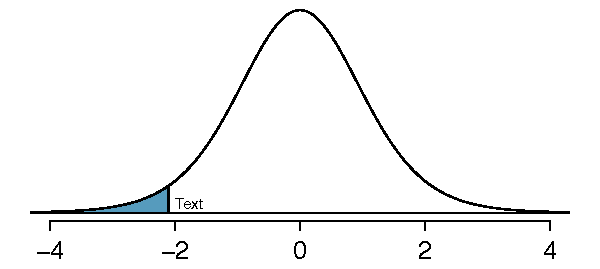
\includegraphics[width=0.5\textwidth]{ch_inference_for_means_oi_biostat/figures/tDistDF18LeftTail2Point10/tDistDF18LeftTail2Point10}
\caption{The $t$-distribution with 18 degrees of freedom. The area below -2.10 has been shaded.}
\label{tDistDF18LeftTail2Point10}
\end{figure}

\end{example}

\newpage

\begin{example}{A $t$-distribution with 20 degrees of freedom is shown in the left panel of Figure~\ref{tDistDF20RightTail1Point65}. Estimate the proportion of the distribution falling above 1.65 and below -1.65.}
Identify the row in the $t$-table using the degrees of freedom: $df-20$. Then, look for 1.65; the value is not listed, and falls between the first and second columns. Since these values bound 1.65, their tail areas will bound the tail area corresponding to 1.65. The two tail area of the first and second columns is between 0.100 and 0.200. Thus, between 10\% and 20\% of the distribution is more than 1.65 standard deviations from the mean. The precise area can be calculated using statistical software: 0.1146.

\begin{figure}
	\centering
	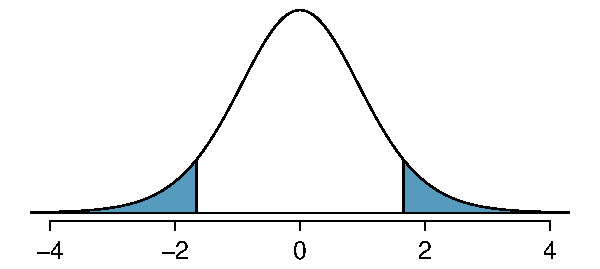
\includegraphics[width=0.5\textwidth]{ch_inference_for_means_oi_biostat/figures/tDistDF20RightTail1Point65/tDistDF20RightTail1Point65}
	\caption{The $t$-distribution with 20 degrees of freedom, with the area further than 1.65 away from 0 shaded.}
	\label{tDistDF20RightTail1Point65}
\end{figure}

\end{example}

\index{t-distribution|)}
\index{distribution!$t$|)}

\subsection{Using the $t$-distribution for tests and confidence intervals for a population mean}

\label{oneSampleTConfidenceIntervalsTests}

\index{t-test!one-sample|(}

Chapter~\ref{foundationsForInference} provided formulas for tests and confidence intervals for population means in random samples large enough for the $t$-statistic to have a nearly normal distribution.  In samples smaller than 30 from approximately symmetric distributions without large outliers, the $t$-statistic has a $t$-distribution with degrees of freedom equal to the sample size - 1. Just like inference in larger samples, inference using the $t$-distribution also requires that the observations in the sample be independent.  Random samples from very large populations always produce independent observations;  in smaller populations, observations will be approximately independent as long as the size of the sample is no larger than 10\% of the population.

Formulas for tests and intervals using the $t-$distribution are very similar to those using the normal distribution.  For a sample of size $n$ with sample mean $\overline{x}$ and standard deviation $s$, two-sided confidence intervals with confidence coefficient $100(1 - \alpha)$\% have the form
\[
    \overline{x} \pm t_{\text{df}}^{\star} \times \text{SE},
\]
where SE is the standard error of the sample mean ($s/\sqrt{n}$) and $t_{\text{df}}^{\star}$ is the point on a $t$-distribution with $n-1$ degrees of freedom and area $(1 - \alpha/2)$ to its right.

A one-sided interval with the same confidence coefficient will have the form  
\begin{align*}
    \overline{x} &+ t_{\text{df}}^{\star} \times \text{SE} \text{   (one-sided upper confidence interval)}, \text{  or} \\
    \overline{x} &- t_{\text{df}}^{\star} \times \text{SE} \text{   (one-sided lower confidence interval)},
\end{align*}
except that in this case $t_{\text{df}}^{\star}$ is the point on a $t$-distribution with $n-1$ degrees of freedom and  area $(1 - \alpha)$ to its right.


\index{data!dolphins and mercury|(}
\begin{example}{Dolphins are at the top of the oceanic food chain; as a consequence, dangerous substances such as mercury tend to be present in their organs and muscles at high concentrations. In areas where dolphins are regularly consumed, it is important to monitor dolphin mercury levels. This example uses data from a random sample of 19 Risso's dolphins from the Taiji area in Japan.\footnote{Taiji is a significant source of dolphin and whale meat in Japan. Thousands of dolphins pass through the Taiji area annually; assume that these 19 dolphins represent a simple random sample. Data reference: Endo T and Haraguchi K. 2009. High mercury levels in hair samples from residents of Taiji, a Japanese whaling town. Marine Pollution Bulletin 60(5):743-747.} Calculate the 95\% confidence for average mercury content in Risso's dolphins from the Taiji area.
		
\begin{table}[h]
	\centering
	\begin{tabular}{ccc cc}
		\hline
		$n$ & $\overline{x}$ & $s$ & minimum & maximum \\
		19   & 4.4	  & 2.3  & 1.7	       & 9.2 \\
		\hline
	\end{tabular}
	\caption{Summary of mercury content in the muscle of 19 Risso's dolphins from the Taiji area. Measurements are in $\mu$g/wet g (micrograms of mercury per wet gram of muscle).}
	\label{summaryStatsOfHgInMuscleOfRissosDolphins}
\end{table}		
		
} %end example

The observations are a simple random sample consisting of less than 10\% of the population, so independence of the observations is reasonable. The summary statistics in Table~\ref{summaryStatsOfHgInMuscleOfRissosDolphins} do not suggest any skew or outliers; all observations are within 2.5 standard deviations of the mean. Based on this evidence, the approximate normality assumption seems reasonable.

Use the $t$-distribution to calculate the confidence interval:
\begin{align*}
\overline{x} \pm  t^{\star}_{\text{df}} \times \text{SE} &= \overline{x}  \pm  t^{\star}_{18}  \times \sqrt{s}/n \\
&= 4.4 \pm  2.10 \times 2.3/\sqrt{19} \\
&= (3.29, 5.51)\,\, \mu\text{g/wet g}.
\end{align*}

The $t^{\star}$ point can be read from the $t$-table on page~\pageref{tTableSample}, in the column with area totaling 0.05 in the two tails (third column) and the row with 18 degrees of freedom. Based on these data, one can be 95\% confident the average mercury content of muscles in Risso's dolphins is between 3.29 and 5.51 $\mu$g/wet gram.

\end{example}

In this example, the $t^{\star}$ point could also have been computed using the function \texttt{qt} in \textsf{R}, which gives the value on the horizontal axis with a specified probability to its left.

\begin{verbatim}
> qt(p = 0.975, df = 18)
[1] 2.100922
\end{verbatim}

\index{data!dolphins and mercury|)}

\begin{exercise} \label{croakerWhiteFishPacificExerConditions}
\index{data!white fish and mercury|(}
The FDA's webpage provides some data on mercury content of various fish species.\footnote{\oiRedirect{textbook-fda_mercury_in_fish_2010}{www.fda.gov/food/foodborneillnesscontaminants/metals/ucm115644.htm}} From a sample of 15 white croaker (Pacific), a sample mean and standard deviation were computed as 0.287 and 0.069 ppm (parts per million), respectively. The 15 observations ranged from 0.18 to 0.41 ppm. Assume that these observations are independent. Based on summary statistics, does the normality assumption seem reasonable? If so, calculate a 90\% confidence interval for the average mercury content of white croaker (Pacific). \footnote{There are no obvious outliers; all observations are within 2 standard deviations of the mean. If there is skew, it is not evident. There are no red flags for the normal model based on this (limited) information. $\overline{x} \ \pm\ t^{\star}_{14} \times SE \ \to\  0.287 \ \pm\  1.76\times 0.0178\ \to\ (0.256, 0.318)$. We are 90\% confident that the average mercury content of croaker white fish (Pacific) is between 0.256 and 0.318 ppm.}
\end{exercise}

\begin{example}{According to the EPA, regulatory action should be taken if fish species are found to have a mercury level of 0.5 ppm or higher. Conduct a formal significance test to evaluate whether the average mercury content of croaker white fish (Pacific) is different from 0.50 ppm. Use $\alpha = 0.05$. 
}

The FDA regulatory guideline is a `one-sided' statement; fish should not be eaten of the mercury level is larger than a certain value.  But without a prior information on whether the mercury in this species tends to be high or low, it is best to do a two-sided test.

State the hypotheses: $H_0: \mu = 0.5$ vs $H_A: \mu \neq 0.5$. Let $\alpha = 0.05$.

Calculate the $t$-statistic: 
\[t = \frac{\overline{x} - \mu_0}{\text{SE}} = \frac{0.287 - 0.50}{0.069/\sqrt{15}} = -11.96\]

The probability that the absolute value of a $t$-statistic with 14 df is smaller than -11.96 is smaller than 0.01. Thus, $p < 0.01$. There is evidence to suggest at the $\alpha = 0.05$ significance level that the average mercury content of this fish species is lower than 0.50 ppm, since $\overline{x}$ is less than 0.50.

\end{example}	

\index{data!white fish and mercury|)}

\index{t-test!one-sample|)}

\section{Paired Data}
\label{pairedData}

\index{paired data|(}
\index{t-test!paired data|(}

In the 2000 Olympics, was the use of a new wetsuit design responsible for an observed increase in swim velocities? In a study designed to investigate this question, twelve competitive swimmers swam 1500 meters at maximal speed, once wearing a wetsuit and once wearing a regular swimsuit.\footnote{De Lucas et. al, The effects of wetsuits on physiological and biomechanical indices during swimming. \textit{Journal of Science and Medicine in Sport,} 2000; 3(1): 1-8} The order of wetsuit versus swimsuit was randomized for each of the 12 swimmers. Table~\ref{swimSuitTimes} shows the average velocity recorded for each swimmer, measured in meters per second (m/s).\footnote{The data are also used in Lock et. al \textit{Statistics, Unlocking the Power of Data}, Wiley, 2013.}

\index{data!swim suit velocities}
% latex table generated in R 3.3.2 by xtable 1.8-2 package
% Wed Sep  6 14:20:56 2017
\begin{table}[ht]
\centering
\begin{tabular}{rrrr}
  \hline
 & swimmer.number & wet.suit.velocity & swim.suit.velocity \\ 
  \hline
1 & 1.00 & 1.57 & 1.49 \\ 
  2 & 2.00 & 1.47 & 1.37 \\ 
  3 & 3.00 & 1.42 & 1.35 \\ 
  4 & 4.00 & 1.35 & 1.27 \\ 
  5 & 5.00 & 1.22 & 1.12 \\ 
  6 & 6.00 & 1.75 & 1.64 \\ 
  7 & 7.00 & 1.64 & 1.59 \\ 
  8 & 8.00 & 1.57 & 1.52 \\ 
  9 & 9.00 & 1.56 & 1.50 \\ 
  10 & 10.00 & 1.53 & 1.45 \\ 
  11 & 11.00 & 1.49 & 1.44 \\ 
  12 & 12.00 & 1.51 & 1.41 \\ 
   \hline
\end{tabular}
\caption{Paired Swim Suit Data} 
\label{swimSuitTimes}
\end{table}

%wet.suit.velocity = c(1.57, 1.47, 1.42, 1.35, 1.22, 
%                      1.75, 1.64, 1.57, 1.56, 1.53, 
%                      1.49, 1.51 )
%swim.suit.velocity = c(1.49, 1.37, 1.35, 1.27, 1.12, 
%                       1.64, 1.59, 1.52, 1.50, 1.45, 
%                       1.44, 1.41)
%swimmer.number = c(1:12)
%swim.suit.study = as.data.frame(cbind(swimmer.number,
%                   wet.suit.velocity, 
%                   swim.suit.velocity))

%swim.suit.study

%xtable(swim.suit.study, caption="Paired Swim Suit Data", 
%       label="swimSuitTimes")
	
The swimsuit velocity data is an example of \term{paired data}, in which two sets of observations  are uniquely paired so that an observation in one set matches an observation in the other; in this case, each swimmer has two measured velocities, one with a wetsuit and one with a swimsuit. A natural measure of the effect of the wetsuit on swim velocity is the difference between the measured maximum velocities (\texttt{diff = wet.suit.velocity - swim.suit.velocity}). Even though there are two measurements per swimmer, using the difference in velocities as the variable of interest allows for the problem to be approached like those in Section~\ref{oneSampleMeansWithTDistribution}.  Although it was not explicitly noted, the data used in Section~\ref{formalHypothesisTesting} were paired; each respondent had both an actual and desired weight.

Suppose the parameter $\delta$ is the population average of the difference in maximum velocities during a 1500m swim if all competitive swimmers recorded swim velocities with each suit type. A hypothesis test can then be conducted with the null hypothesis that there is no difference population average swim velocities, $H_0: \delta = 0$, against the alternative that there is a difference, $H_A: \delta \neq 0$.

\begin{termBox}{\tBoxTitle{Stating hypotheses for paired data}
When testing a hypothesis about paired data, compare the groups by testing whether the true mean difference between the groups is equal to 0.
\begin{itemize}
\item For a two-sided test, $H_0: \delta = 0$; $H_A: \delta \neq 0$.
\item For a one-sided test, either $H_0: \delta = 0$; $H_A: \delta > 0$ or  $H_0: \delta = 0$; $H_A: \delta < 0$.
\end{itemize}
}
\end{termBox}

Some important assumptions are being made. First, the data are a random sample from the population. While the observations are likely independent, it is more difficult to justify that this sample of 12 swimmers is randomly drawn from the entire population of competitive swimmers. Nevertheless, it is often assumed in problems such as these that the participants are reasonably representative of competitive swimmers. Second, it is assumed that the population of differences is normally distributed. This is a small sample, one in which normality would be difficult to confirm. The dot plot for the difference in velocities is shown in Figure~\ref{swimmerDotPlot}; shows approximate symmetry and a boxplot can be used to show there are no outliers.


\begin{figure}[h]
	\centering
	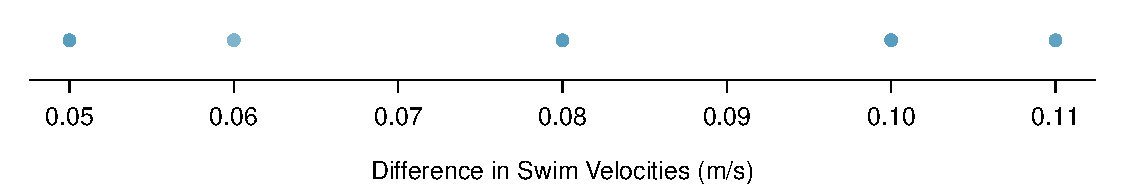
\includegraphics[width=0.9\textwidth]{ch_inference_for_means_oi_biostat/figures/swimDotPlot/swimDotPlot}
	\caption{A dot plot of differences in swim velocities.}
	\label{swimDotPlot}
\end{figure}

Let $\overline{x}_{\text{diff}}$ denote the sample average of the differences in maximum velocity, $s$ the sample standard deviation of the differences, and $n$ the number of pairs in the dataset. The $t$-statistic used to test $H_0$ vs. $H_A$ is: 

\[\frac{\overline{x}_{\text{diff}} - \delta_0} {s_{\text{diff}}/\sqrt{n}},\]

where in this case $\delta_0 = 0$.\footnote{This value is specified by the null hypothesis of no difference.}

\begin{example}{Using the data in Table~\ref{swimSuitTimes}, conduct a two-sided hypothesis test at $\alpha = 0.05$ to assess whether there is evidence to suggest that wetsuits have an effect on swim velocities during a 1500m swim.}

The hypotheses are $H_0: \delta = 0$ and $H_A: \delta \neq 0$. Let $\alpha = 0.05$. 

Calculate the $t$-statistic:

\[t = \frac{\overline{x}_{\text{diff}} - \delta_0} {s_{\text{diff}}/\sqrt{n}} = \frac{0.078 - 0}{0.022/\sqrt{12}} = 12.32\]

The two-sided $p$-value is
$$ p = P(T < -\text{12.32}) + P(T > \text{12.32}), $$
where $T$ is a $t$-distributed random variable with $n-1 = 11$  degrees of freedom.
The $t$-table shows that $p < 0.01$. Software can be used to show that $p = (2.3)(10^{-7}$, a very small value indeed. If software was used to calculate the $p$-value, it would be sufficient to note that $2 < 0.001$. 
	
The data support the claim that the wetsuits changed swim velocity in a 1500m swim. The observed average increase of 0.078~m/s is significantly different than the null hypothesis of no change, and suggests that swim velocities are higher when swimmers wear wetsuits as opposed to swimsuits.	

\end{example}

\index{t-test!paired data|)}

Calculating confidence intervals for paired data also involves calculating the differences between the values in each pair, then applying the same approach as for single-sample data. For example, a two-sided 95\% confidence interval for paired data has the form:

\[ \left(
  \overline{x}_{\text{diff}} - t^\star_{df} \times \frac{s_{\text{diff}}}{\sqrt{n}},
  \:\: \overline{x}_{\text{diff}} + t^\star_{df} \times \frac{s_{\text{diff}}}{\sqrt{n}} \right), 
\] 

where $t^\star$ is the point on a $t$ distribution with $df = n - 1$ for $n$ pairs, with area 0.025 to its right.

\begin{exercise} 
Using the data in Table~\ref{swimSuitTimes}, calculate a 95\% confidence interval for the average difference in swim velocities during a 1500m swim. Is the interval consistent with the results of the hypothesis test?\footnote{Use the values of $\overline{x}_{\text{diff}}$ and $s_{\text{diff}}$ as calculated previously: 0.078 and 0.022. The $t^\star$ value of 2.20 has $df = 11$ and 0.025 area to the right. The confidence interval is ($0.078 \pm \frac{0.022}{\sqrt{12}}$) $\to$ (0.064, 0.091) m/s. With 95\% confidence, $\delta$ lies between 0.064 m/s and 0.09 m/s. The interval does not include 0 (no change), which is consistent with the result of the hypothesis test.}
\end{exercise}

The general approach when analyzing paired data is to first calculate the differences between the values in each pair, then use those differences in methods for confidence intervals and tests for a single sample.  Any conclusion from an analysis should be stated in terms of the original paired measurements.


%__________________
\section{Difference of two means}
\label{differenceOfTwoMeans}





Does treatment using embryonic stem cells (ESCs) help improve heart function following a heart attack? New and potentially risky treatments are sometimes tested in animals before studies in humans.  In  2005 paper in \textit{Lancet}\footnote{ Lancet 2005; 366: 1005–12 } Menard, et al. describe an experiment in 18 sheep with induced heart attacks were randomly assigned to receive either ESCs transplanted in the heart or to receive inert material in the transplant.  Various measures of cardiac function were measured 1 month after the transplant.

This design is typical of an interventional study. Statistically, this is the problem of drawing inference about the difference in two population means, $\mu_1 - \mu_2$, when the data are not paired. The point estimate of the difference, $\overline{x}_1 - \overline{x}_2$, is used to calculate a $t$-statistic that is the basis of confidence intervals and tests.


\subsection{Confidence interval for a difference of means}
\label{confidenceIntervalDifferenceMeans}

\index{data!stem cells, heart function|(}
\index{point estimate!difference of means|(}

Table~\ref{summaryStatsForSheepHeartDataWhoReceivedMiceESCs} contains summary statistics for the 18 sheep, 9 in each group.  The data is in the data set \data{stem.cells} in the \textsf{R} package OpenIntro. Each sheep was randomly assigned to either the control or experimental group, and percent change in heart pumping capacity measured. A positive value corresponds to increased pumping capacity, which generally suggests a stronger recovery from the heart attack.  This section illustrates the confidence intervals that can be used to examine the evidence for a potential treatment effect when using stem cells to in sheep with a heart attack. 


\begin{table}[h]
\centering
\begin{tabular}{l rrrrr}
\hline
\hspace{10mm}	& $n$	& $\overline{x}$	& $s$  	 \\
\hline
ESCs		& 9		& 3.50		& 5.17  	\\
control		& 9		& -4.33		& 2.76  	 \\
\hline
\end{tabular}
\caption{Summary statistics of the embryonic stem cell study.}
\label{summaryStatsForSheepHeartDataWhoReceivedMiceESCs}
\end{table}

\begin{figure}[h]
	\centering
	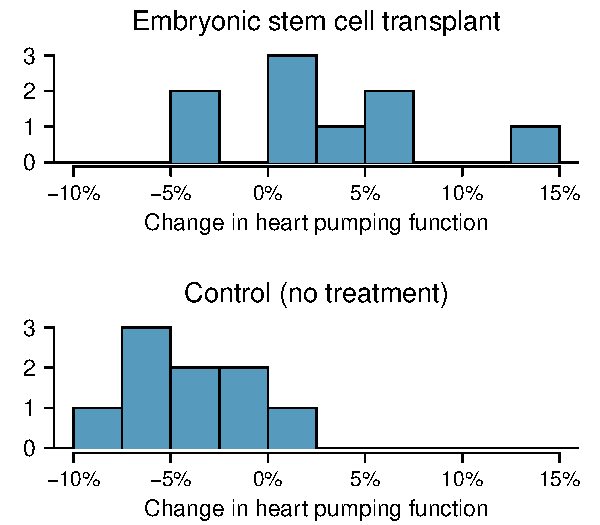
\includegraphics[width=0.58\textwidth]{ch_inference_for_means_oi_biostat/figures/stemCellTherapyForHearts/stemCellTherapyForHearts}
	\caption{Histograms for both the embryonic stem cell group and the control group. Higher values are associated with greater improvement.}
	\label{stemCellTherapyForHearts}
\end{figure}

Figure~\ref{stemCellTherapyForHearts} shows that the distributions of percent change do not have any prominent outliers, which would indicate a deviation from normality; this suggests that each sample mean can be modeled using a $t$-distribution. Additionally, the sheep in the study were independent of each other, and the sheep between groups are also independent. Thus, the $t$-distribution can be used to model the difference of the two sample means.

\begin{termBox}{\tBoxTitle{Using the $t$-distribution for a difference in means}
\label{ConditionsForTwoSampleTDist}The $t$-distribution can be used for inference when working with the standardized difference of two means if (1) each sample meets the conditions for using the $t$-distribution and (2) the samples are independent.}
\end{termBox}

\index{point estimate!difference of means|)}

A confidence interval for a difference of two means has the same basic structure as previously discussed confidence intervals:

\[(\overline{x}_{1} - \overline{x}_{2}) \pm t^\star_{df} \times \text{ SE }. \]

\index{standard error (SE)!difference in means}

The following formula is used to calculate the standard error of $\overline{x}_{1} - \overline{x}_{2}$. Since $\sigma$ is typically unknown, the standard error is estimated by using $s$ in place of $\sigma$. 

\[
SE_{\overline{x}_{1} - \overline{x}_{2}} = \sqrt{\frac{\sigma_{1}^2}{n_{1}} + \frac{\sigma_{2}^2}{n_{2}}} \approx \sqrt{\frac{s_{1}^2}{n_{1}} + \frac{s_{2}^2}{n_{2}}}.
\]

In this setting, the $t$-distribution has a somewhat complicated formula for the degrees of freedom that is usually calculated with software\footnote{See the end of chapter notes for the formula}. An alternative approach uses the smaller of $n_1 - 1$ and $n_2 - 1$ as the degrees of freedom.\footnote{This technique for degrees of freedom is conservative with respect to a Type~1 Error; it is more difficult to reject the null hypothesis using this formula for $df$.}

\begin{termBox}{\tBoxTitle{Distribution of a difference of sample means}
The sample difference of two means, $\overline{x}_1 - \overline{x}_2$, can be modeled using the $t$-distribution and the standard error
\begin{eqnarray}
\textstyle
SE_{\overline{x}_{1} - \overline{x}_{2}} = \sqrt{\frac{s_1^2}{n_1} + \frac{s_2^2}{n_2}}
\label{seOfDifferenceInMeans}
\end{eqnarray}
when each sample mean can itself be modeled using a $t$-distribution and the samples are independent. To calculate the degrees of freedom without using software, use statistical software or the smaller of $n_1 - 1$ and $n_2 - 1$.}
\end{termBox}%\textC{\vspace{-10mm}}

\begin{example}{Calculate a 95\% confidence interval for the effect of ESCs on the change in heart pumping capacity of sheep following a heart attack.}
	
Calculate the point estimate for the difference: $\overline{x}_1 - \overline{x}_2 = \overline{x}_{\text{esc}} - \overline{x}_{\text{control}} = 7.83$.	
	
Calculate the standard error: 	

\[\sqrt{\frac{s_{1}^2}{n_{1}} + \frac{s_{2}^2}{n_{2}}} = \sqrt{\frac{5.17^2}{9} + \frac{2.76^2}{9}} = 1.95\]
	
Since $n_1 = n_2 = 9$, use $df = 8$; $t^{\star}_{8} = 2.31$ for a 95\% confidence interval. Alternatively, computer software can provide a more accurate value for degrees of freedom, $df = 12.225$.

The confidence interval is given by:

\[(\overline{x}_{1} - \overline{x}_{2}) \pm t^\star_{df} \times \text{ SE } \quad\rightarrow\quad
7.83 \ \pm\ 2.31\times 1.95 \quad\rightarrow\quad (3.38, 12.38) \]

With 95\% confidence, the average amount that ESCs improve heart pumping capacity lies between 3.38\% to 12.38\%.
\end{example}

\index{data!stem cells, heart function|)}


\subsection{Hypothesis tests for a difference in means}
\label{testingDifferenceMeans}


\index{t-test!two independent groups|(}

\index{data!baby\_smoke|(}

Is there evidence that newborns from mothers who smoke have a different average birth weight than newborns from mothers who do not smoke? The dataset \data{baby\_smoke} contains data from a random sample of 150 cases of mothers and their newborns in North Carolina over a year; there are 50 cases in the smoking group and 100 cases in the nonsmoking group.

\begin{table}[h]
\centering
\begin{tabular}{rrrrrll}
  \hline
 & fAge & mAge & weeks & weight & sexBaby & smoke \\ 
  \hline
1 & NA & 13 &  37 & 5.00 & female & nonsmoker \\ 
  2 & NA & 14 &  36 & 5.88 & female & nonsmoker \\ 
  3 & 19 & 15 &  41 & 8.13 & male & smoker \\ 
  $\vdots$ &   $\vdots$ &   $\vdots$ &   $\vdots$ &   $\vdots$ &   $\vdots$ \\
  150 & 45 & 50 &  36 & 9.25 & female & nonsmoker \\ 
   \hline
\end{tabular}
\caption{Four cases from the \data{baby\_smoke} dataset.}
\label{babySmokeDF}
\end{table}

\begin{example} {Evaluate whether it is appropriate to apply the $t$-distribution to the difference in sample means between the two groups.}
Since the data come from a simple random sample and consist of less than 10\% of all such cases, the observations are independent. While each distribution is strongly skewed, the large sample sizes of 50 and 100 allow for the use of the $t$-distribution to model each mean separately. Thus, the difference in sample means may be modeled using a $t$-distribution.	
\end{example}

\begin{figure}[hhh]
\centering
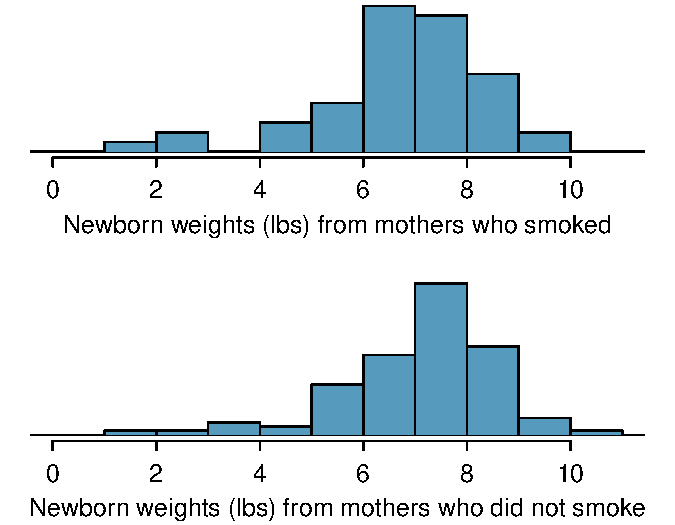
\includegraphics[width=0.63\textwidth]{ch_inference_for_means_oi_biostat/figures/babySmokePlotOfTwoGroupsToExamineSkew/babySmokePlotOfTwoGroupsToExamineSkew}
\caption{The top panel represents birth weights for infants whose mothers smoked. The bottom panel represents the birth weights for infants whose mothers who did not smoke. The distributions exhibit moderate-to-strong and strong~skew, respectively.\index{skew!example: strong}}
\label{babySmokePlotOfTwoGroupsToExamineSkew}
\end{figure}

A hypothesis test can be conducted to evaluate whether there is a relationship between mother's smoking status and average newborn birth weight. The null hypothesis represents the case of no difference between the groups, $H_0: \mu_{ns} - \mu_{s} = 0$, where $\mu_{ns}$ represents the population mean of newborn birthweight for non-smoking mothers, and $\mu_s$ represents mean newborn birthweight for mothers who smoke. Under the alternative hypothesis, there is some difference in average newborn birth weight between the groups, $H_A: \mu_{ns} - \mu_{s} \neq 0$. The hypotheses can also be written as $H_0: \mu_{ns} = \mu_{s}$ and $H_A: \mu_{ns} \neq \mu_{s}$.

\begin{termBox}{\tBoxTitle{Stating hypotheses for two-group data}
When testing a hypothesis about two independent groups, directly compare the two population means and state hypotheses in terms of $\mu_1$ and $\mu_2$.
\begin{itemize}
	\item For a two-sided test, $H_0: \mu_{1} = \mu_{2}$; $H_A: \mu_{1} \neq \mu_{2}$.
	\item For a one-sided test, either $H_0: \mu_{1} = \mu_{2}$; $H_A: \mu_{1} > \mu_{2}$ or  $H_0: \mu_{1} = \mu_{2}$; $H_A: \mu_{1} < \mu_{2}$.
\end{itemize}
	}
\end{termBox}


In this setting, the formula for a $t$-statistic is:

\[t = \dfrac{(\overline{x}_1 - \overline{x}_2) - (\mu_1 - \mu_2)}{SE_{\overline{x}_{1} - \overline{x}_{2}}} = \dfrac{(\overline{x}_1 - \overline{x}_2) - (\mu_1 - \mu_2)}{\sqrt{\dfrac{s_{1}^{2}}{n_1} + \dfrac{s_{2}^{2}}{n_2}}} \]

Under the null hypothesis of no difference between the groups, $H_0: \mu_{1} - \mu_{2} = 0$, the formula simplifies to

\[t = \dfrac{(\overline{x}_1 - \overline{x}_2)}{\sqrt{\dfrac{s_{1}^{2}}{n_1} + \dfrac{s_{2}^{2}}{n_2}}}\]

\begin{example}{Conduct a hypothesis test on the \data{baby\_smoke} data to evaluate whether there is evidence that newborns from mothers who smoke have a different average birth weight than newborns from mothers who do not smoke. 
		
\begin{table}[hhh]
	\centering
	\begin{tabular}{lrr}
		& \resp{smoker} & \resp{nonsmoker} \\
		\hline
		mean & 6.78 & 7.18 \\
		st. dev. & 1.43 & 1.60 \\
		samp. size & 50 & 100 \\
		\hline
	\end{tabular}
	\caption{Summary statistics for the \data{baby\_\hspace{0.3mm}smoke} data set.}
	\label{summaryStatsOfBirthWeightForNewbornsFromSmokingAndNonsmokingMothers}
\end{table}		

}

The hypotheses are $H_0: \mu_{1} = \mu_{2}$ and $H_A: \mu_{1} \neq \mu_{2}$, where $\mu_{1}$ represents the average newborn birth weight for nonsmoking mothers and $\mu_{2}$ represents average newborn birth weight for mothers who smoke. Let $\alpha = 0.05$. 	

Calculate the $t$-statistic:

\[t = \dfrac{(\overline{x}_1 - \overline{x}_2)}{\sqrt{\dfrac{s_{1}^{2}}{n_1} + \dfrac{s_{2}^{2}}{n_2}}} = \dfrac{7.18 - 6.78}{\sqrt{\frac{1.60^2}{100} + \frac{1.43^2}{50}}} = 1.54\]

Approximate the degrees of freedom as $50 - 1 = 49$. The $t$-score of 1.49 falls between the first and second columns in the $df = 49$ row of the $t$-table, so the two-sided $p$-value is between 0.10 and 0.20. The \textsf{R} function \texttt{pt} can be used to find a more precise version of the $p$-value.
\begin{verbatim}
2*pt(q = 1.49, df = 49, lower.tail = FALSE)
[1] 0.1426335
\end{verbatim}

This $p$-value is larger than the significance value, 0.05, so the null hypothesis not rejected. There is insufficient evidence to state there is a difference in average birth weight of newborns from North Carolina mothers who did smoke during pregnancy and newborns from North Carolina mothers who did not smoke during pregnancy.
\end{example}

\index{t-test!two independent groups|)}

\subsection{The paired $t$-test vs. two independent groups}
\label{pairedVsTwoGroups}

Students often find it difficult to determine whether a paired $t$-test or a test for two independent groups should be used.  The paired test applies only in situations where there is a natural pairing between the observations in the two groups, such as in the swim suit data.  Pairing should be one of the first things to look for in the data. Pairing can be obvious, such as the two measurements for each swimmer, or more subtle, such as measurements of respiratory function in twins, where one member of the twin pair was treated with an experimental treatment and the other with a control.  In the case of two independent groups, the two group sizes are often different, so comparing sample sizes can help with the distinction.   When the two sample sizes are equal, there should be no natural way to pair the observations.

A common error when data are paired is to assume the two groups are independent and conduct a two-group $t$-test.  The swim suit data can be used to show the possible harm in making that error.  In Section~\ref{pairedData}, the paired $t$-test showed a significant difference in the swim velocities between wet suits and regular swim suits. Suppose the analysis had been conducted using a two independent group test, ignoring the fact that the measurements were paired.

The mean and standard deviation for the 12 wet suit velocities are 1.51 and 0.14 (both m/sec), respectively, and 1.43 and 0.14 (m/sec) for the 12 swim suit velocities. A two-group $t-test$ has value
\begin{align*}
	t &= \frac{1.52 - 1.43}{\sqrt{0.14^2/12 + 0.14^2/12}} \\
	  &= 1.37 
\end{align*}
If the degrees of freedom can be approximated by 11 = 12 - 1, the two-sided p-value from software is 0.20.  Using this method the null hypothesis of equal mean velocities for the two suit types would not be rejected.

It is not difficult to show that the numerator of the paired $t$-test (the average of the within swimmer differences) and the numerator of the two-group test (the difference of the average times for the two groups) are identical.  The different values of the test statistics arise because the standard errors used to calculate the statistics are different.  For the paired test, the standard error uses the standard deviation of the within pair differences (0.22) and has value $0.022/\sqrt{12} = 0.006$.  The two-group test combines the standard deviations for the original measurements and has value $\sqrt{0.14^2/12 + 0.14^2/12} = 0.06$.  The standard error for the two-group test is 10-fold larger than for the paired test.  This striking difference in the standard errors is caused by the much smaller variability of the individual velocity differences compared to the variability of the original measurements.  This shows the value of pairing, when it is appropriate to do so.  Because of the correlation between the within swimmer velocities the two velocities for each swimmer are close to each other and the differences are consistently small, producing low variability.

The swim suit data illustrates a difficulty that often arises in statistics; both the paired and two-group tests are numerically correct, and each can be calculated either by hand or in software without an apparent error.  But the context of the problem dictates that the paired test is a correct approach, while the two-group test is incorrect.

\subsection{Case study: discrimination in developmental disability support}

\index{data!developmental disability support|(}

Section~\ref{caseStudyDiscrimination} introduced the dataset \data{dds.discr}, which examined expenditures for supporting developmentally disabled residents in the state of California, by age and ethnicity. The analysis presented in that section explored the confounding in that dataset.  When the variable \var{age} is ignored, the expenditures per consumer for is larger on average for White non-Hispanics than Hispanics, but Table~\ref{ddsAvgExpEthAge} showed that average differences by ethnicity were much smaller within age cohorts.  This section uses $t$-tests to conduct a more formal analysis of possible differences in expenditure by ethnicity, both overall (i.e., ignoring age) and within age cohorts. 

Figure~\ref{ddsEthnicityPlot} shows that, when ignoring age, expenditures within the ethnicity groups Hispanic and White non-Hispanic show substantial right-skewing. Figure~\ref{ddsLogExpenditureEthnicityPlot)} contains side-by-side boxplots of the natural logarithm of expenditures by ethnicity.  The natural log transformation has effectively eliminated the skewing, so it is prudent to conduct a $t$-test for differences in expenditures overall by ethnicity on the transformed data.

\begin{figure}[h]
	\centering
	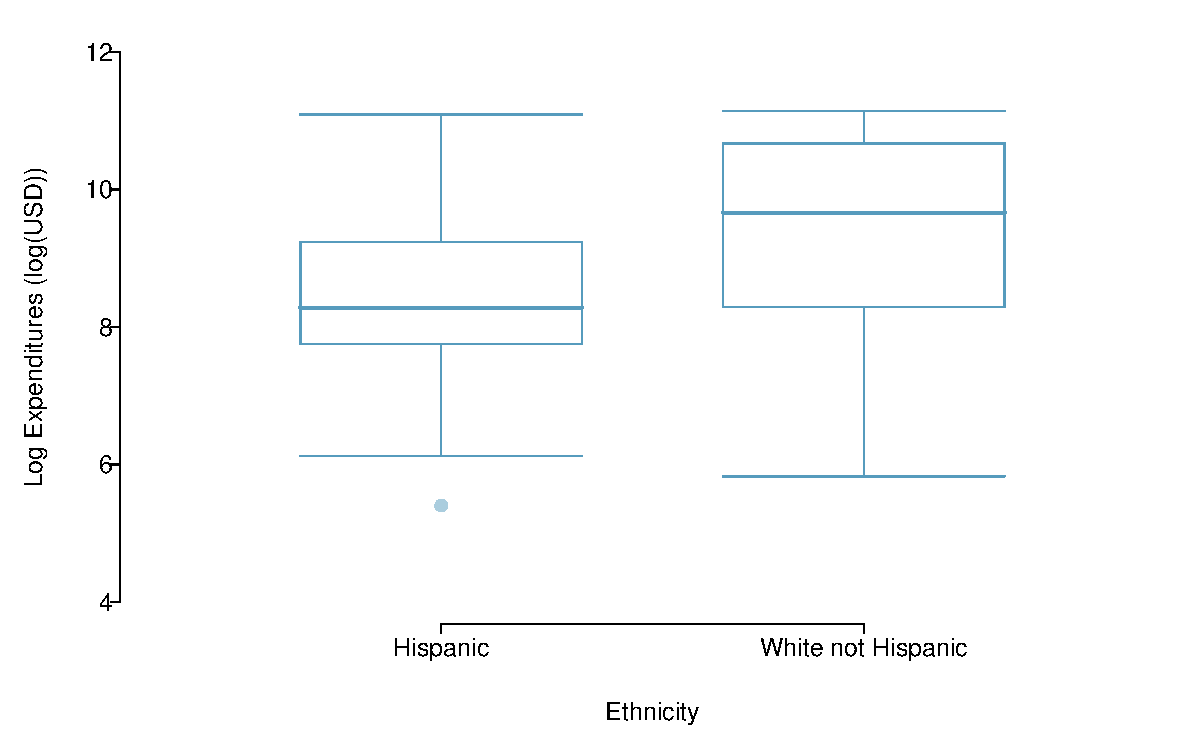
\includegraphics[width=0.99\textwidth]{ch_inference_for_means_oi_biostat/figures/ddsLogExpEthnicityPlot/ddsLogExpEthnicityPlot.pdf}
	\caption{A plot of \texttt{log(expenditures)} by \texttt{ethnicity}.}
	\label{ddsLogExpEthnicityPlot}
\end{figure} 



The first $t$-test is a test of the null hypothesis $H_0: \mu_{\text{Hispanic}} = \mu_{\text{White non-Hispanic}}$ vs. the two-sided alternative  $H_A: \mu_{\text{Hispanic}} \neq \mu_{\text{White non-Hispanic}}$, where $\mu$ is the population mean log expenditure within an ethnicity group. Table~\ref{ddsLogExpenditureSummaryByEthnicity} contains the summary statistics for the transformed variable $\log(\texttt{expenditures})$ needed to calculate a $t$-test for differences by ethnicity.

% dt = data.frame(dds.hisp.white$ethnicity, dds.hisp.white$log.expenditures)
% dt$ethnicity = dt$dds.hisp.white.ethnicity
% dt$log.expenditures = dt$dds.hisp.white.log.expenditures
% xtable(ddply(dt, ~ethnicity, summarise, Cases = length(log.expenditures), Mean = mean(log.expenditures),StdDev = sd(log.expenditures)))
% latex table generated in R 3.3.2 by xtable 1.8-2 package
% Wed Oct 25 10:51:17 2017

\begin{table}[ht]
\centering
\begin{tabular}{rlrrr} \hline
 & Ethnicity & Cases & Mean & StdDev \\  \hline
1 & Hispanic & 376 & 8.56 & 1.17 \\ 
2 & White not Hispanic & 401 & 9.47 & 1.35 \\  \hline
\end{tabular}
\label{ddsLogExpenditureSummaryByEthnicity} 
\end{table}

The $t$-statistic for the test is 

\begin{align*}
  t &= \frac{9.47 - 8.56}{\sqrt{1.35^2/401 + 1.17^2/376}} \\
    &=10.1
 \end{align*}

The smaller of the two sample sizes - 1 is 375, so the degrees of freedom is large enough to use a normal approximation for the $p$-value. But whether one uses the $t$ or the normal distribution, the probability that a $t$-statistic has has absolute value larger than 10 is vanishingly small, so the p-value is less than 0.001. As indicated in Section~\ref{caseStudyDiscrimination}, however, this difference, no matter how significant, can be misleading, since the differences in expenditure are smaller within age cohorts than when age is ignored. Age is a confounding variable in this setting

While the average differences within age cohorts are smaller, they might still suggest discrimination if the differences are larger than would be expected by chance alone.  Table~\ref{ddsEthAgeTable} shows that the age cohort 13-17 is the largest among the Hispanic consumers, while the cohort 22-50 is the largest among White non-Hispanics. This section uses $t$-tests to examine the evidence against the null hypothesis of no difference in average payments within these two cohorts.

Figure~\ref{ddsExpEthnicityAge13} shows that within the age cohort 13-17, the distribution of payments is reasonably symmetric within the two groups Hispanic and White non-Hispanic.  This was evident in the Figures~\ref{ddsExpAge} and \ref{ddsExpEthnicity}; within age cohorts, expenditures were not skewed, but are skewed within ethnicity groups.  The skewing evident when age was ignored was caused by the different distribution of ages within the ethnicities. Because of the approximate symmetry of expenditures in this age cohort, the log transform used in the overall analysis is not necessary to insure the validity of the $t$-test.


\begin{figure}[h]
	\centering
	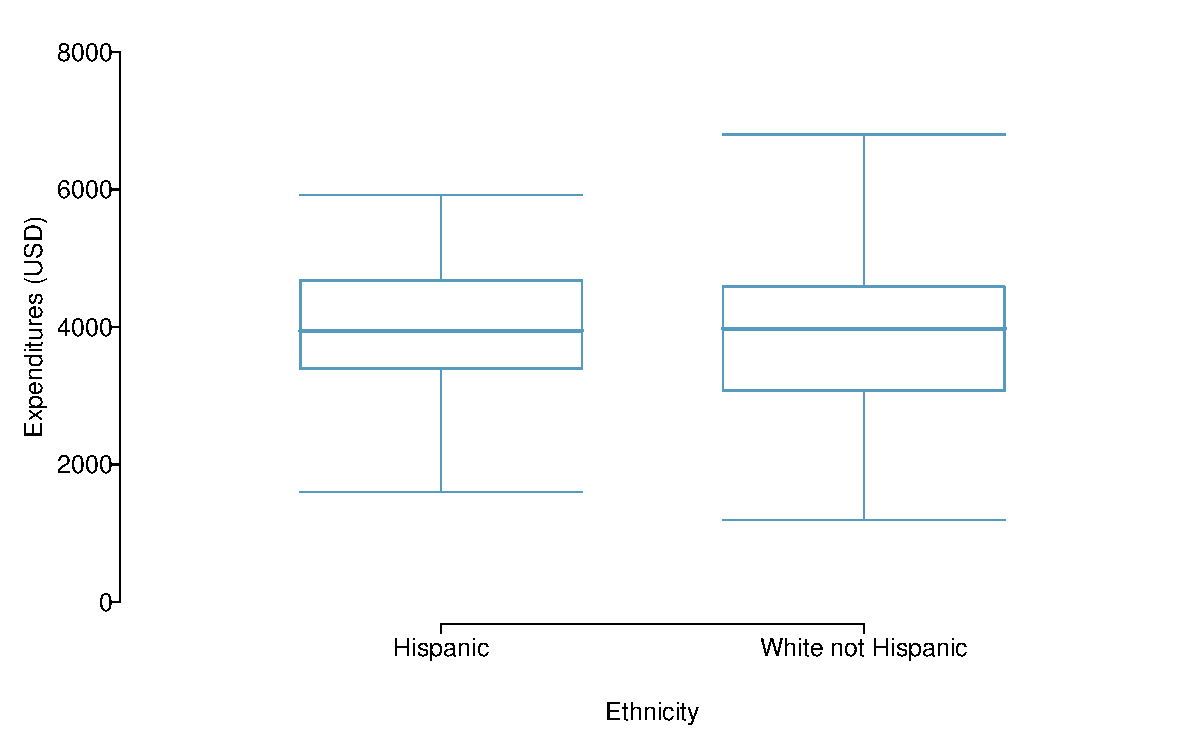
\includegraphics[width=0.99\textwidth]{ch_inference_for_means_oi_biostat/figures/ddsExpEthnicityAge13/ddsExpEthnicityAge13}
	\caption{A plot of \texttt{expenditures} by \texttt{ethnicity} in the age cohort 13 - 17. }
	\label{ddsExpEthnicityAge13}
\end{figure} 


Table~\ref{ddsExpenditureSummaryByEthnicityAge13} contains the summary statistics used in computing the $t$-statistic for comparing expenditures in the two groups within this age cohort.  The $t$ statistic has value $t = 0.318$, with degrees of freedom 66 and non-significant two-sided p-value $p=0.75$.

% dt.13$Ethnicity = dt.13$ethnicity
% dt.13$Ethnicity = dt.13$ethnicity
% xtable(ddply(dt.13, ~ethnicity, summarise, Cases = length(expenditures), Mean =
% mean(expenditures),StdDev = sd(expenditures)),+       caption = ``Summary statistics for Expenditures,
% Age 13-17'',`label = ``ddsExpenditureSummaryByEthnicity.Age13'')
% latex table generated in R 3.3.2 by xtable 1.8-2` package
% Mon Oct 30 11:16:30 2017
\begin{table}[ht]
  \centering
  \begin{tabular}{rlrrr}  \hline
& Ethnicity & Cases & Mean & StdDev \\   \hline
1 & Hispanic & 103 & 3955.28 & 938.82 \\ 
2 & White not Hispanic &  67 & 3904.36 & 1071.02 \\    
\hline
\end{tabular}
\caption{Summary statistics for Expenditures, Age 13-17}
\label{ddsExpenditureSummaryByEthnicity.Age13}
\end{table}

The analysis of the age cohort 22 - 50 shows the same qualitative result.  The side-by-side boxplots of expenditures (Figure~\ref{ddsExpEthnicityAge22}) show approximate symmetry, and the $t$-statistic calculated from the summary statistics in Table~\ref{ddsExpEthnicityAge22} has value $t = 0.659$ and is not significant.


\begin{figure}[h]
	\centering
	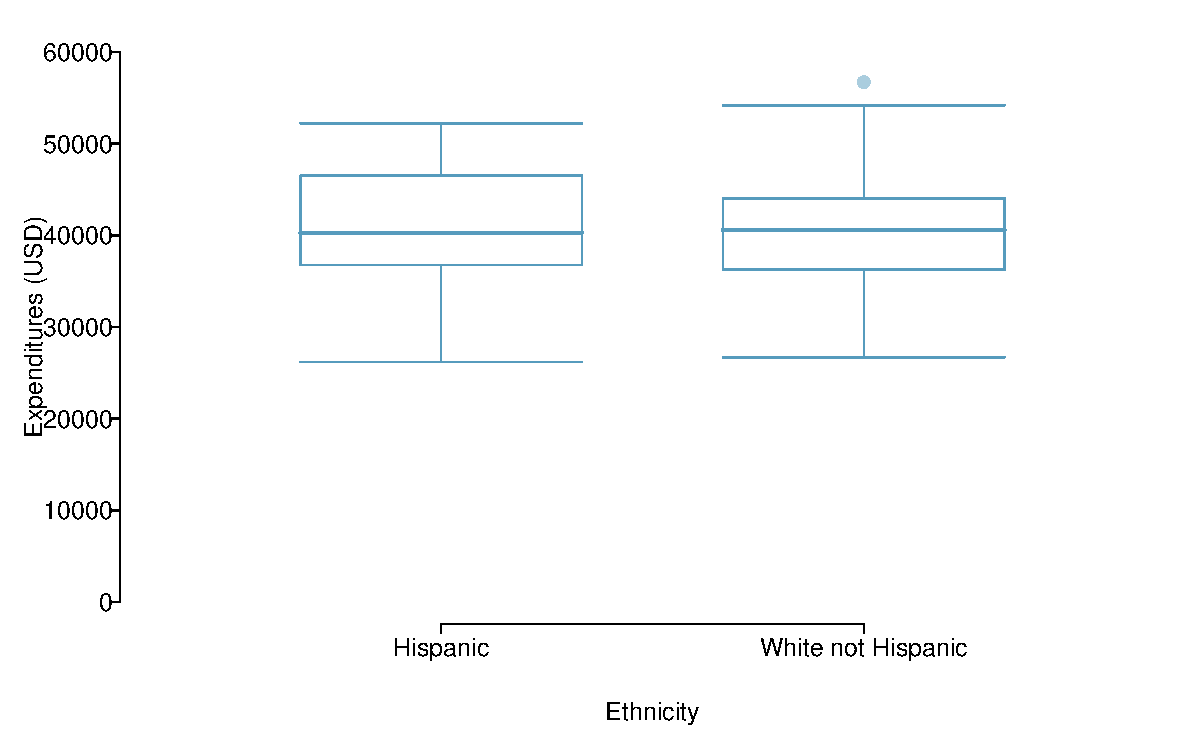
\includegraphics[width=0.99\textwidth]{ch_inference_for_means_oi_biostat/figures/ddsExpEthnicityAge22/ddsExpEthnicityAge22}
	\caption{A plot of \texttt{expenditures} by \texttt{ethnicity} in the age cohort 22 - 50. }
	\label{ddsExpEthnicityAge22}
\end{figure} 



%dt.22 = subset(dds.hisp.white, age.cohort == "22-50", select = c(ethnicity, expenditures))
% xtable(ddply(dt.22, ~ethnicity, summarise, Cases = length(expenditures),Mean = mean(expenditures), StdDev = sd(expenditures)),caption = "Summary statistics for Expenditures, Age 22 - 50", label = "ddsExpenditureSummaryByEthnicity.Age22")
% latex table generated in R 3.3.2 by xtable 1.8-2 package
% Mon Oct 30 11:50:18 2017
\begin{table}[ht]
\centering
\begin{tabular}{rlrrr}
  \hline
 & Ethnicity & Cases & Mean & StdDev \\ 
  \hline
1 & Hispanic &  43 & 40924.12 & 6467.09 \\ 
  2 & White not Hispanic & 133 & 40187.62 & 6081.33 \\ 
   \hline
\end{tabular}
\caption{Summary statistics for Expenditures, Age 22 - 50} 
\label{ddsExpenditureSummaryByEthnicity.Age22}
\end{table}


\index{data!developmental disability support|)}



\subsection{Pooled standard deviation estimate (special topic)}
\label{pooledStandardDeviations}

Occasionally, two populations will have standard deviations that are so similar that they can be treated as identical. For example, historical data or a well-understood biological mechanism may justify this strong assumption. In such cases, it can be more precise to use a pooled standard deviation to make inferences about the difference in population means.

The \term{pooled standard deviation} of two groups uses data from both samples to estimate the common standard deviation and the standard error. If there are good reasons to believe that the population standard deviations are equal, an improved estimate of the group variances can be obtained by pooling the data from the two groups:
\begin{align*}
s_{\text{pooled}}^2 = \frac{s_1^2 (n_1-1) + s_2^2 (n_2-1)}{n_1 + n_2 - 2},
\end{align*}
where $n_1$ and $n_2$ are the sample sizes, and $s_1$ and $s_2$ represent the sample standard deviations. In this setting, the $t$-statistic uses $s_{\text{pooled}}^2$ in place of $s_1^2$ and $s_2^2$ in the standard error formula. In this setting, the degrees of freedom for the $t-$statistic is the sum of the degrees of freedom for the two sample variances:
\[
\text{df} = (n_1 - 1) + (n_2 - 1) = n_1 + n_2 - 2.
\]
The $t$-statistic for testing the null hypothesis of no difference between population means becomes 
\[
 t = \frac{\overline{x}_1 - \overline{x}_2}{s_{\text{pooled}}\sqrt{\frac{1}{n_1} + \frac{1}{n_2}}}. 
\]

The formula for the two-sided confidence interval for the difference in population means is
\[
(\overline{x}_1 - \overline{x}_2) \pm t^{\star} \times s_p \sqrt{\frac{1}{n_1} + \frac{1}{n_2}},
\]
where $t^{\star}$ is the point on a $t$-distribution with $n_1 + n_2 -2$ degrees of freedom chosen according to the confidence coefficient.

The benefits of pooling the standard deviation are realized through obtaining a better estimate of the standard deviation for each group and using a larger degrees of freedom parameter for the $t$-distribution. Both of these changes may permit a more accurate model of the sampling distribution of $\overline{x}_1 - \overline{x}_2$, if the standard deviations of the two groups are indeed equal.  In most applications, however, it is difficult to verify the assumption of equal population standard deviations, and thus safer to use the methods discussed in Sections~\ref{confidenceIntervalDifferenceMeans} and \ref{testingDifferenceMeans}.

%__________________
\section[Power calculations for a difference of means (special topic)]{Power calculations for a difference of means\\ (special topic)}
\label{PowerForDifferenceOfTwoMeans}

Designing a study often involves many complex issues, most of which cannot be covered in this text. Perhaps the most important statistical issue in study design is the choice an appropriate sample size. The \term{power} of a statistical test is the probability that the test will reject the null hypothesis when the alternative hypothesis is true; sample sizes are chosen to make that probability sufficiently large, typically between 80\% and 90\%. Practitioners often use the term `detecting' a difference to mean correctly rejecting a null hypothesis, i.e., rejecting a null hypothesis when the alternative is true.

Two competing considerations arise when choosing a sample size. The sample size should be sufficiently large to allow for important group differences to be detected in a hypothesis test. If a study is so small that detecting a statistically significant difference is unlikely even when there are potentially important differences, enrolling participants might be unethical, since subjects could potentially be exposed to a dangerous experimental treatment. However, it is also unethical to conduct studies with an overly large sample size, since more participants than necessary would be exposed to an intervention with uncertain value. Collecting data is also usually expensive and time consuming.

This section begins by illustrating relevant concepts in the context of a hypothetical clinical trial, where the goal is to calculate a sufficient sample size for being 80\% likely to detect practically important effects.\footnote{While sample size planning is also important for observational studies, those techniques are not discussed here.} Afterwards, formulas are provided for directly calculating sample size, as well as references to software that can perform the calculations.

\subsection{Reviewing the concepts of a test}

\begin{example}{The company would like to run the clinical trial with participants whose systolic blood pressures are between 140 and 180 mmHg. Suppose previously published studies suggest that the standard deviation of the patients' blood pressures will be about 12 mmHg, with an approximately symmetric distribution.\footnote{In many studies like this one, each participant's blood pressure would be measured at the beginning and end of the study, and the outcome measurement for the study would be the average difference in blood pressure in each of the treatment groups. For this hypothetical study, we assume for simplicity that blood pressure is measured at only the end of the study, and that the randomization ensures that blood pressures at the beginning of the study are equal (on average) between the two groups.} What would be the approximate standard error for $\overline{x}_{ \text{trmt}} - \overline{x}_{ \text{ctrl}}$ if 100 participants were enrolled in each treatment group?}
The standard error is calculated as follows:
\begin{align*}
SE_{\overline{x}_{ \text{trmt}} - \overline{x}_{ \text{ctrl}}}
  = \sqrt{\frac{s_{ \text{trmt}}^2}{n_{ \text{trmt}}} + \frac{s_{ \text{ctrl}}^2}{n_{ \text{ctrl}}}}
  = \sqrt{\frac{12^2}{100} + \frac{12^2}{100}}
  = 1.70.
\end{align*}
This may be an imperfect estimate of $SE_{\overline{x}_{ \text{trmt}} - \overline{x}_{\text{ctrl}}}$, since the standard deviation estimate of 12 mmHg from prior data may not be correct. However, it is sufficient for getting started, and making an assumption like this is often the only available option. 
\end{example}

Since the degrees of freedom are greater than 30, the distribution of $\overline{x}_{ \text{trmt}} - \overline{x}_{ \text{ctrl}}$ will be approximately normal. Under the null hypothesis, the mean is 0 and the standard deviation is 1.70 (from the standard error).

\begin{center}
	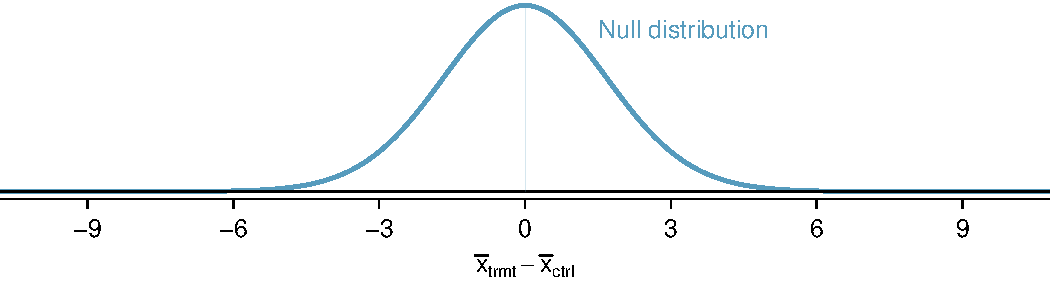
\includegraphics[width=0.93\textwidth]{ch_inference_for_means_oi_biostat/figures/power_null_0_1-7/power_null_A_0_1-7}
\end{center}


\begin{example}{For what values of $\overline{x}_{\text{trmt}} - \overline{x}_{\text{ctrl}}$ would the the null hypothesis be rejected, using $\alpha = 0.05$?}
If the observed difference is in the far left or far right tail of the null distribution, there is sufficient evidence to reject the null hypothesis.
For $\alpha = 0.05$, $H_0$ is rejected if the difference is in the lower 2.5\% or upper 2.5\% tail:
\begin{description}
\setlength{\itemsep}{0mm}
\item[Lower 2.5\%:] For the normal model, this is 1.96 standard errors below 0, so any difference smaller than $-1.96 \times 1.70 = -3.332$~mmHg.
\item[Upper 2.5\%:] For the normal model, this is 1.96 standard errors above 0, so any difference larger than $1.96 \times 1.70 = 3.332$~mmHg.
\end{description}
The boundaries of these \term{rejection regions} are shown below. Note that if the new treatment is effective, mean blood pressure should be lower in the treatment group than in the control group; i.e., the difference should be in the lower tail.
\begin{center}
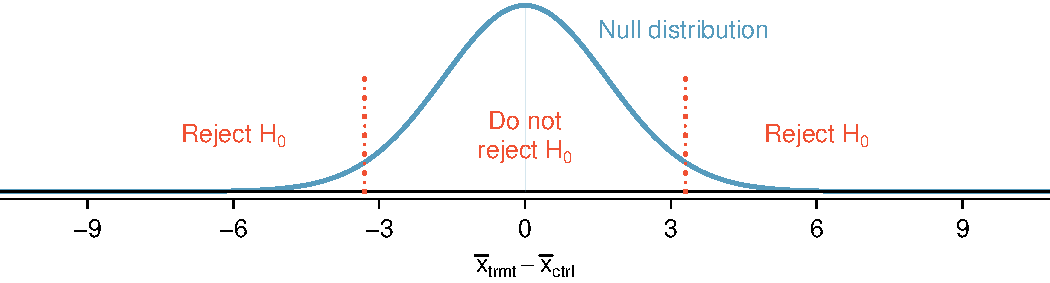
\includegraphics[width=0.93\textwidth]{ch_inference_for_means_oi_biostat/figures/power_null_0_1-7/power_null_B_0_1-7_with_rejection_region}
\end{center}
\end{example}

The next step is to perform some hypothetical calculations to determine the probability of rejecting the null hypothesis if the alternative hypothesis were true.

\subsection{Computing the power for a 2-sample test}

If there is a real effect from an intervention, and the effect is large enough to have practical value, the probability of detecting that effect is referred to as the \term{power}. Power can be computed for different sample sizes or different effect sizes. 

There is no easy way to define when an effect size is large enough to be of value; this is not a statistical issue. For example, in a clinical trial, the scientifically significant effect would be the incremental value of the intervention that would justify changing current clinical recommendations from an existing intervention to a new one. In this case, the effect size is usually determined from long discussions between the research team and study sponsors. 

Suppose that for this hypothetical blood pressure medication study, the researchers are interested in detecting any effect on blood pressure that is 3 mmHg or larger than the standard medication. Here, 3 mmHg is the minimum \term{population effect size} of interest. 

\begin{example}{Suppose the study proceeded with 100 patients per treatment group and the new drug does reduce average blood pressure by an additional 3~mmHg relative to the standard medication. What is the probability that of detecting this effect?}\label{PowerFor100AtNeg3}

Determine the sampling distribution for $\overline{x}_{\text{trmt}} - \overline{x}_{\text{ctrl}}$ when the true difference is $-3$~mmHg; this has the same standard deviation of 1.70 as the null distribution, but the mean is shifted 3 units to the left. Then, calculate the fraction of the distribution for $\overline{x}_{\text{trmt}} - \overline{x}_{\text{ctrl}}$ that falls within the rejection region for the null distribution.

\begin{figure}[h]
\begin{center}
	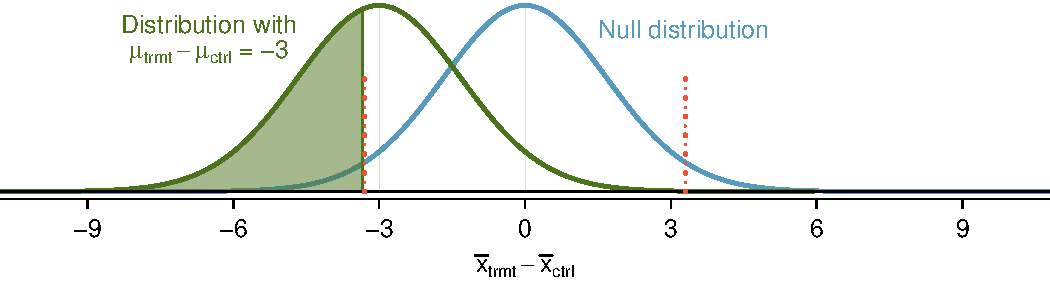
\includegraphics[width=0.87\textwidth]{ch_inference_for_means_oi_biostat/figures/power_null_0_1-7/power_null_D_0_1-7_with_alt_at_3_and_shaded}
	\caption{The rejection regions are outside of the dotted lines. Recall that the boundaries for $\alpha = 0.05$ were calculated to be $\pm 3.332$ mmHg.}
\end{center}	
\end{figure}

The probability of being in the left side of the rejection region ($x < -3.332$) can be calculated by converting to a $Z$-score and using either the normal probability table or statistical software.\footnote{The probability of being in the right side of the rejection region is negligible and can be ignored.}

\[
	Z = \frac{-3.332 - (-3)}{1.7}= -0.20 \quad \to \quad P(Z \leq -0.20) = 0.4207
\]

The power for the test is about 42\% when $\mu_{\text{trmt}} - \mu_{\text{ctrl}} = -3$~mm/Hg and each group has a sample size of 100.
\end{example}



\subsection{Determining a proper sample size}

The last example demonstrated that with a sample size of 100 in each group, there is a probability of about 0.42 of detecting an effect size of 3~mmHg. If the study were conducted with this sample size, even if the new medication reduced blood pressure by 3~mmHg compared to the control group, there is a less than 50\% chance of concluding that the medication is beneficial. Studies with low power are often inconclusive, and there are important reasons to avoid such a situation:

\begin{itemize}
	\setlength{\itemsep}{0mm}
	\item Participants were subjected to the drug but the study may have little scientific value. A study with 100 participants per group using a drug that does lower blood pressure by 3~mmHG is more likely than not to fail to reject the null hypothesis of no treatment effect, but failure to reject the null hypothesis does not prove there is no effect.
	
	\item The company may have invested hundreds of millions of dollars in developing the new drug, and may now left with uncertainty about its potential.
	
	\item Another clinical trial may need to be conducted to obtain a more conclusive answer as to whether the drug does hold any practical value, and that would require substantial time and expense. 
\end{itemize}

To ensure a higher probability of detecting a clinically important effect, a higher sample size should be chosen. What about a study with 500 patients per group?

%JV: cannot resize the graphical parameters because there is an R error that appears when running the original OI code...

\begin{exercise}
Calculate the power to detect a change of -3~mmHg  using a sample size of 500 per group. Recall that the standard deviation was expected to be about 12 mmHg.\footnote{(a) The standard error will now be $SE = \sqrt{\frac{12^2}{500} + \frac{12^2}{500}} = 0.76$.\\
(b) The null distribution, rejection boundaries, and alternative distribution are shown below. The rejection regions are the areas on outside the two dotted lines at $\pm 0.76 \times 1.96 = \pm 1.49$. \\
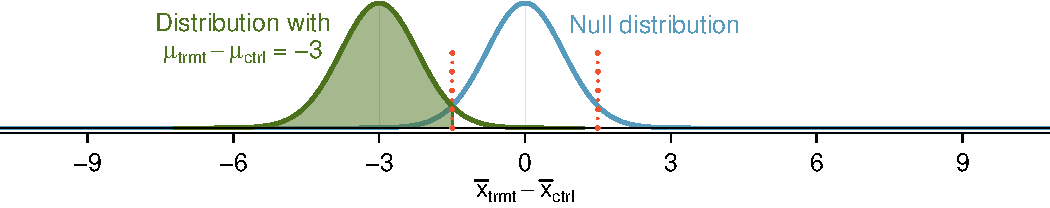
\includegraphics[width=0.9\textwidth]{ch_inference_for_means_oi_biostat/figures/power_null_0_0-76/power_null_0_0-76_with_alt_at_3_and_shaded} \\
(c) Compute the $Z$-score and find the tail area, $Z = \frac{-1.49 - (-3)}{0.76} = 1.99 \to P(Z \leq 1.99) = 0.9767$, which is the power of the test for a difference of 3 mmHg. With 500 patients per group, the study would be 97.7\% likely to detect an effect size of 3~mmHg.}
\begin{enumerate}[(a)]
\setlength{\itemsep}{0mm}
\item Determine the standard error.
\item Identify the null distribution and rejection regions, as well as the alternative distribution when $\mu_{trmt} - \mu_{ctrl} = -3$.
\item Compute the probability of rejecting the null hypothesis.
\end{enumerate}
\end{exercise}

With a sample size of 500 per group, the power of the test is much larger than necessary. Not only does this lead to a study that would be overly expensive and time consuming, it also exposes more patients than necessary to the experimental drug. 

Sample sizes are generally chosen such that power is around 80\%, although in some cases 90\% is the target. Other values may be reasonable for a specific context, but 80\% and 90\% are most commonly chosen as a good balance between high power and limiting the number of patients exposed to a new treatment (as well as reducing experimental costs). 

\begin{example}{Identify the sample size that would lead to a power of 80\%.}

The $Z$-score that defines a lower tail area of 0.80 is about $Z = 0.84$. In other words, 0.84 standard errors from -3, the mean of the alternative distribution. 

\begin{center}
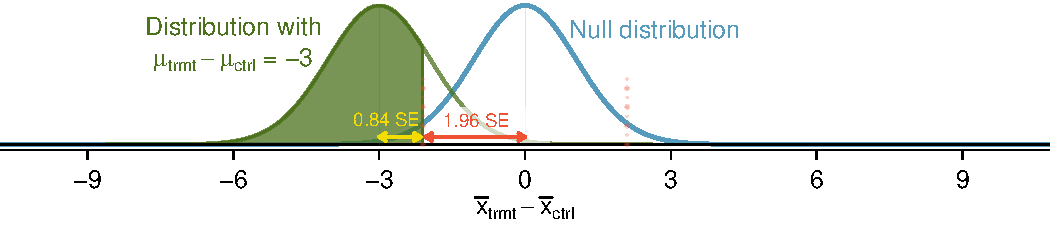
\includegraphics[width=0.93\textwidth]{ch_inference_for_means_oi_biostat/figures/power_best_sample_size/power_best_sample_size}
\end{center}

For $\alpha = 0.05$, the rejection region always extends 1.96 standard errors from 0, the center of the null distribution. 

The distance between the centers of the null and alternative distributions can be expressed in terms of the standard error:
\begin{align*}
(0.84 \times SE) + (1.96 \times SE) = 2.8 \times SE.
\end{align*}

This quantity necessarily equals the minimum effect size of interest, 3 mmHg, which is the distance between -3 and 0. It is then possible to solve for $n$:
\begin{align*}
3 &= 2.8 \times SE \\
3 &= 2.8 \times \sqrt{\frac{12^2}{n} + \frac{12^2}{n}} \\
% 3^2 &= 2.8^2 \times \left( \frac{12^2}{n} + \frac{12^2}{n} \right) \\
n &= \frac{2.8^2}{3^2} \times \left( 12^2 + 12^2 \right) = 250.88 \\
\end{align*}
The study should enroll about 251 patients per group.
\end{example}

\begin{exercise}
Suppose the targeted power is 90\% and $\alpha = 0.01$. How many standard errors should separate the centers of the null and alternative distributions, where the alternative distribution is centered at the minimum effect size of interest? Assume the test is two-sided.\footnote{Find the $Z$-score such that 90\% of the distribution is below it: $Z = 1.28$. Next, find the cutoffs for the rejection regions: $\pm 2.58$. Then the difference in centers should be about $1.28 \times SE + 2.58 \times SE = 3.86 \times SE$.}
\end{exercise}

Figure~\ref{power_curve_neg-3} shows the power for sample sizes from 20~participants to 5,000~participants when $\alpha = 0.05$ and the true difference is -3 mmHg. Having more than 250-300 observations does not provide much additional value in detecting an effect. 

\begin{figure}[h]
\centering
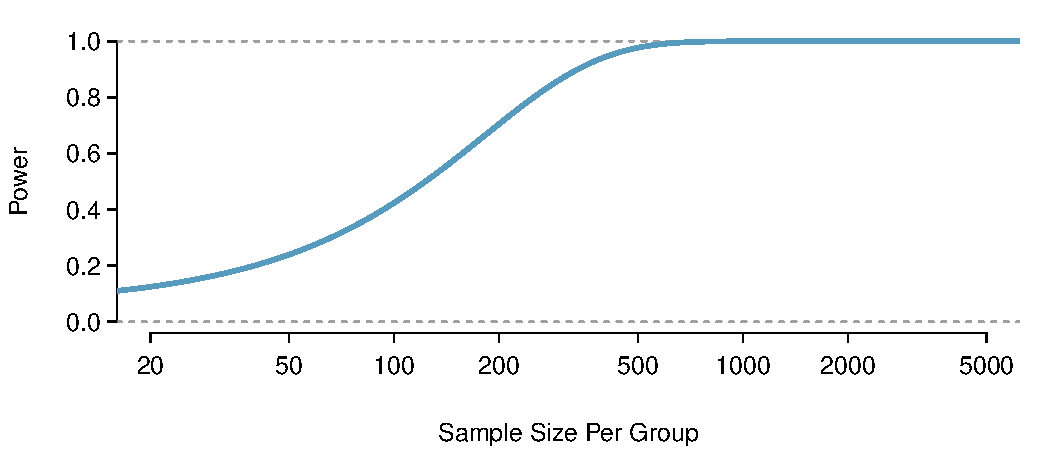
\includegraphics[width=0.9\textwidth]{ch_inference_for_means_oi_biostat/figures/power_curve/power_curve_neg-3}
\caption{The curve shows the power for different sample sizes in the context of the blood pressure example when the true difference is -3.}
\label{power_curve_neg-3}
\end{figure}

\subsection{Formulas for power and sample size}

Power and sample size calculations are so important that it is generally prudent not to use the previously illustrated methods of deriving them from first principles. Instead, there are many commercially available and public domain programs that should be the method of choice. In the early stages of planning a study, however, hand calculations using formulas can provide a quick estimate.

Use the following formula to calculate sample size for comparing two means, assuming each group will have $n$ participants:

\[
n = \frac{(\sigma_1^2 + \sigma_2^2)( z_{1-\alpha/2} + z_{1-\beta})^2}
{\Delta^2}.
\]

In this formula: 
\begin{itemize}
\setlength{\itemsep}{0mm}
	
	\item $\mu_1, \sigma_1, \mu_2, \text{ and } \sigma_2$ are the population means and standard deviations of the two groups.
	
	\item $\Delta = \mu_1 - \mu_2$ is the minimally important difference that investigators wish to detect.
	
	\item The null and alternative hypotheses are $H_0: \Delta = 0$ (i.e., no difference between the means) and $H_A: \Delta \neq 0$, i.e., a two-sided alternative.
	
	\item The two-sided significance level is $\alpha$, and $z_{1-\alpha/2}$ is the point on a standard normal distribution with area $1-\alpha/2$ to its left and $\alpha/2$ area to its right.
	
	\item $\beta$ is the probability of incorrectly failing to reject $H_0$ for a specified value of $\Delta$, and that $1- \beta$ is the power.  The value $z_{1-\beta}$ is the point on a standard normal distribution with area $1 - \beta$ to its left.
	
\end{itemize}


For a study with sample size $n$ per group, where $Z$ is a normal random variable with mean 0 and standard deviation 1, power is given by:
\[
	\text{Power } = P\left(  Z <-z_{1 - \alpha/2} + \frac{\Delta}
	{\sqrt{\sigma_1^2/n + \sigma_2^2/n}}\right).
\]

These formulas could have been used in the earlier power and sample size calculations for the hypothetical study of blood pressure lowering medication. To calculate the sample size needed for 80\% power in detecting a change of 3 mmHg, $\alpha = 0.05$, $1 - \beta = 0.80$, $\Delta = 3$ mmHg, and $\sigma_1 = \sigma_2 = 12$ mmHg. The formula yields a sample size $n$ per group of 
\[n = \frac{(12^2 + 12^2)(1.96 + 0.84)^2}{(-3.0)^2} = 250.88, \]
which can be rounded up to 251.

The formula for power can be used to verify the sample size of 251:
\begin{align*}
	\text{Power } &= P\left(Z < -1.96 + \frac{3}
	{\sqrt{12^2/251 + 12^2/251}}\right) \\
	&= P(Z < 1.25) \\
	&= 0.85.
\end{align*}
The calculated power is slightly larger than 80\% because of the rounding to 251.

When designing and conducting a study, the sample size calculations done before any data are collected are one of the most critical aspects of study design. If an analysis is done incorrectly, it can be redone once the error is discovered. However, if data were collected for a sample size that is either too large or too small, it can be impossible to correct the error, especially in studies with human subjects. As a result, sample size calculations are nearly always done using software. For two-sample $t$-tests, the \textsf{R} function \texttt{power.t.test} is both freely available and easy to use, as illustrated in the \textsf{R} companion to this text.

\section[Comparing more than two means with ANOVA (special topic)]{Comparing many means with ANOVA\\(special topic)}
\label{anovaAndRegrWithCategoricalVariables}

\index{analysis of variance (ANOVA)|(}

In some settings, it is useful to compare means across several groups. It might be tempting to do pairwise comparisons between groups; for example, if there are three groups ($A, B, C$), why not conduct three separate $t$-tests ($A$ vs. $B$, $A$ vs. $C$, $B$ vs. $C$)? Conducting multiple tests on the same data increases the rate of Type I error, however, making it more likely that a difference will be found by chance, even if there is no difference among the population means. 

Instead, the methodology behind a $t$-test can be generalized to a procedure called \term{analysis of variance (ANOVA)}, which uses a single hypothesis test to assess whether the means across many groups are equal. Strong evidence favoring the alternative hypothesis in ANOVA is described by unusually large differences among the group means.


\begin{itemize}
	\setlength{\itemsep}{0mm}
	\item[$H_0$:] The mean outcome is the same across all groups. In statistical notation, $\mu_1 = \mu_2 = \cdots = \mu_k$ where $\mu_i$ represents the mean of the outcome for observations in category $i$.
	\item[$H_A$:] At least one mean is different.
\end{itemize}

There are three conditions on the data that must be checked before performing ANOVA: 1) observations are independent within and across groups, 2) the data within each group are nearly normal, and 3) the variability across the groups is about equal.

\begin{example}{Examine Figure~\ref{toyANOVA}. Compare groups I, II, and III. Is it possible to visually determine if the differences in the group centers is due to chance or not? Now compare groups IV, V, and VI. Do these differences appear to be due to chance?
		
\begin{figure}[h]
	\centering
	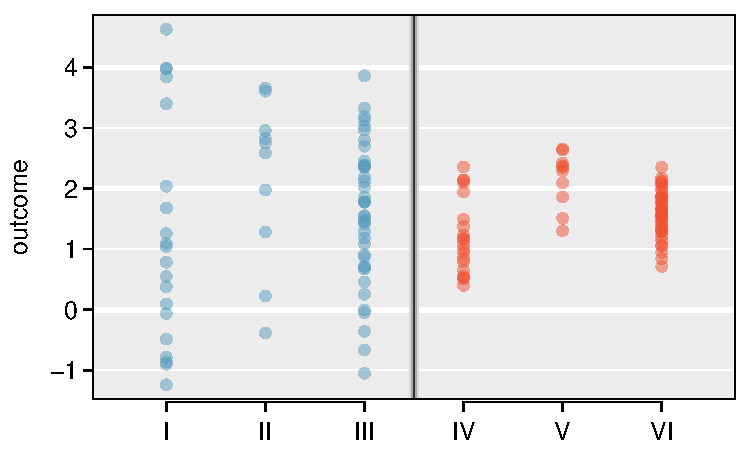
\includegraphics[width=0.68\textwidth]{ch_inference_for_means_oi_biostat/figures/toyANOVA/toyANOVA}
	\caption{Side-by-side dot plot for the outcomes for six groups.}
	\label{toyANOVA}
\end{figure}		

}
	
	It is difficult to discern a difference in the means of groups I, II, and III, because the data within each group are very variable relative to any differences in the average outcome. However, there appear to be differences in the centers of groups IV, V, and VI. For instance, group V appears to have a higher mean than that of the other two groups. The differences in centers for groups IV, V, and VI are noticeable because those differences are large relative to the variability in the individual observations within each group.
\end{example}

\subsection{Analysis of variance (ANOVA) and the F test}
\label{ANOVASection}

Fhe \data{famuss} dataset was introduced in Chapter~\ref{introductionToData}, Section~\ref{variableTypes}. In the FAMuSS study, researchers examined the relationship between muscle strength and genotype at a location on the ACTN3 gene. Descriptions for each variable are provided in Table~\ref{famussVariables}, reproduced below. The measure for muscle strength (the outcome variable) is percent change in strength in the non-dominant arm (\var{ndrm.ch}). Is there a difference in muscle strength across the three genotype categories (\texttt{CC}, \texttt{CT}, {TT})?

\begin{table}[h]
	\centering\small
	\begin{tabular}{lp{10.5cm}}
		\hline
		{\bf variable} & {\bf description} \\
		\hline
		\var{sex} & Sex of the participant \\
		\var{age} & Age in years   \\
		\var{race} & Recorded as African Am (African American), Caucasian, Asian, Hispanic and Other \\
		\var{height} & Height in inches    \\
		\var{weight} & Weight in pounds \\
		\var{actn3.r577x} & Genotype at the location r577x in the ACTN3 gene. \\
		\var{ndrm.ch} & Percent change in strength in the non-dominant arm, comparing strength after to before training \\
		\hline
	\end{tabular}
	\caption{Variables and their descriptions for the \data{famuss} dataset.\vspaceB{-3.5mm}}
\end{table}

\begin{exercise} \label{nullHypForFamuss}
	The null hypothesis under consideration is the following: $\mu_{\resp{CC}} = \mu_{\resp{CT}} = \mu_{\resp{TT}}$.
	Write the null and corresponding alternative hypotheses in plain language.\footnote{$H_0$: The average percent change in non-dominant arm strength is equal across the three genotypes. $H_A$: The average percent change in non-dominant arm strength varies across some (or all) groups.}
\end{exercise}

Table~\ref{famussSummaryTable} provides summary statistics for each group. A side-by-side boxplot for the change in non-dominant arm strength is shown in Figure~\ref{famussBoxPlot}. Notice that the variability appears to be approximately constant across groups; nearly constant variance across groups is an important assumption that must be satisfied for using ANOVA. It seems reasonable to assume normality; while there are some outliers in each group, this is not a concern since the sample sizes are relatively large.

\begin{table}[ht]
	\centering\small
	\begin{tabular}{lrrr}
		\hline
		& \resp{CC} & \resp{CT} & \resp{TT} \\
		\hline
		Sample size ($n_i$)	& 173 & 261 & 161 \\
		Sample mean ($\bar{x}_i$)	& 48.89 & 53.25 & 58.08 \\
		Sample SD ($s_i$)	& 29.96 & 33.23 & 35.69 \\
		\hline
	\end{tabular}
	\caption{Summary statistics of change in non-dominant arm strength, split by genotype.}
	\label{famussSummaryTable}
\end{table}


\begin{figure}[h]
	\centering
	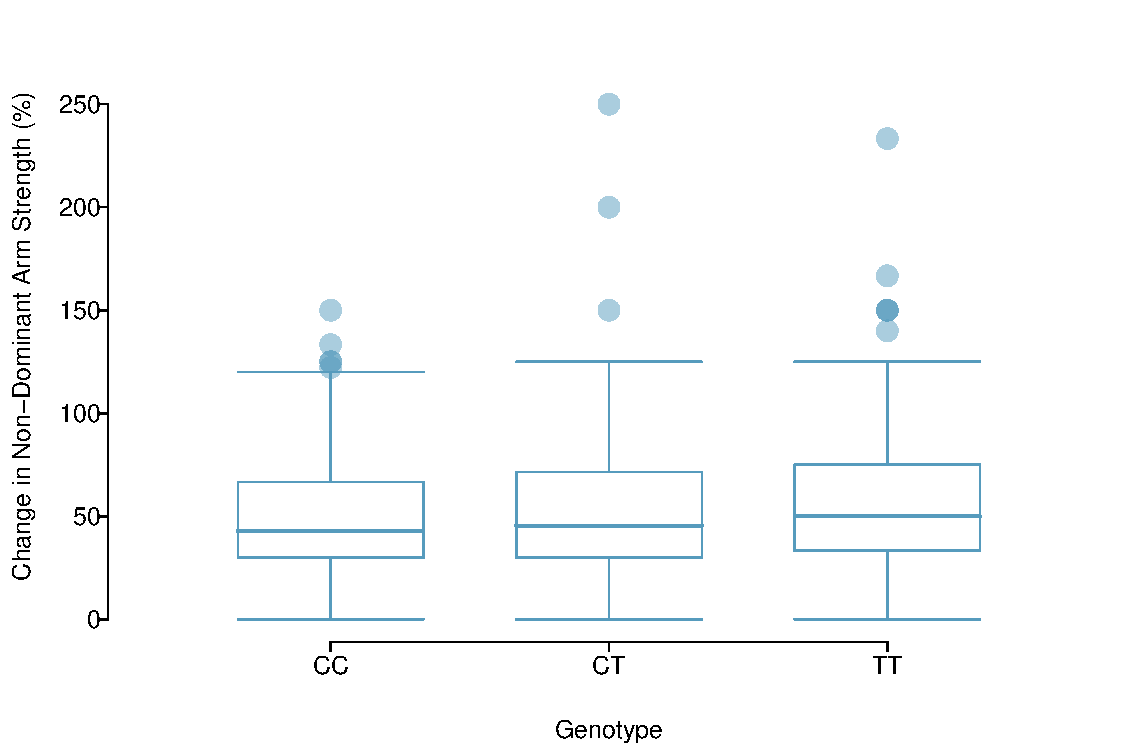
\includegraphics[width=0.7\textwidth]{ch_inference_for_means_oi_biostat/figures/famussBoxPlot/famussBoxPlot}
	\caption{Side-by-side box plot of the change in non-dominant arm strength for 595 participants across three groups.}
	\label{famussBoxPlot}
\end{figure}

\begin{example}{The largest difference between the sample means is between the \texttt{CC} and \texttt{TT} groups. Consider again the original hypotheses:
		\begin{itemize}
			\setlength{\itemsep}{0mm}
			\item[$H_0$:] $\mu_{\resp{CC}} = \mu_{\resp{CT}} = \mu_{\resp{TT}}$
			\item[$H_A$:] The average percent change in non-dominant arm strength ($\mu_i$) varies across some (or all) groups.
		\end{itemize}
		Why might it be inappropriate to run the test by simply estimating whether the difference of $\mu_{\var{CC}}$ and $\mu_{\resp{TT}}$ is statistically significant at a 0.05 significance level?}
	\label{multipleComparisonExample}
	
	It is inappropriate to informally examine all data and decide which groups to formally test. This is a form of \term{data fishing}; choosing the groups with the largest differences for the formal test will lead to an inflation in the Type~I error rate. Instead, all the groups should be tested using a single hypothesis test.
\end{example}

Analysis of variance focuses on answering one question: is the variability in the sample means large enough that it seems unlikely to be from chance alone? This involves simultaneously considering several groups, and evaluating whether their sample means differ more than would be expected from natural variation. This variability is referred to as the \term{mean square between groups ($MSG$)}, which has an associated degrees of freedom $df_{G}=k-1$ when there are $k$ groups. Essentially, the $MSG$ is a measure of how much each group mean varies from the overall mean. Let $\overline{x}$ represent the mean of outcomes across all groups. Then the mean square between groups is computed as:

\[MSG = \frac{1}{df_{G}}SSG = \frac{1}{k-1}\sum_{i=1}^{k} n_{i}\left(\bar{x}_{i} - \bar{x}\right)^{2},\] 

where $SSG$ is called the \term{sum of squares between groups} and $n_{i}$ is the sample size of group $i$. 

%JV: Trying to clearly pin down the logic for comparing between-group and within-group variation.

Under the null hypothesis, any observed variation in group means is due to chance and there is no real difference between the groups. In other words, the null hypothesis assumes that the groupings are non-informative, such that all observations can be thought of as belonging to a single group. If this scenario is true, then it is reasonable to expect that the variability between the group means should be equal to the variability observed within a single group. The \term{mean square error ($MSE$)} is a pooled variance estimate with associated degrees of freedom $df_E=n-k$ that provides a measure of variability within the groups. the mean square error is computed as:

\[MSE = \frac{1}{df_{E}}SSE = \frac{1}{n-k}\sum_{i=1}^{k} (n_i-1)s_i^{2}, \]

where the $SSE$ is the \term{sum of squared errors}, $n_i$ is the sample size of group $i$, and $s_i$ is the standard deviation of group $i$.

When the null hypothesis is true, any differences among the sample means are only due to chance, and the $MSG$ and $MSE$ should be equal. The test statistic for ANOVA, the \term{F statistic}, is the ratio of the between-group variability to the within-group variability:

\begin{align} \label{formulaForTheFStatistic}
F = \frac{MSG}{MSE}
\end{align}


\begin{example}{Calculate the $F$ statistic for the \data{famuss} data summarized in Table~\ref{famussSummaryTable}. The overall mean $\overline{x}$ across all observations is 53.29.}
 
First, calculate the $MSG$ and $MSE$. 
\vspace{0mm}
\begin{align*}
MSG =& \frac{1}{k-1}\sum_{i=1}^{k} n_{i}\left(\bar{x}_{i} - \bar{x}\right)^{2} \\
=& \frac{1}{3-1} [(173)(48.89 - 53.29)^{2} + (261)(53.25 - 53.29)^{2} + (161)(58.08 - 53.29)^{2} ]\\
=& 3521.69 \\
MSE =& \frac{1}{n-k}\sum_{i=1}^{k} (n_i-1)s_i^{2} \\
=& \frac{1}{595-3}[(173-1)(29.96^2) + (261-1)(33.23^2) + (161-1)(35.69^2)] \\
=& 1090.02
\end{align*}

The $F$ statistic is the ratio:

\[\dfrac{MSG}{MSE} = \dfrac{3521.69}{1090.02} = 3.23 \]

\end{example} 

A $p$-value can be computed from the $F$ statistic using an $F$ distribution, which has two associated parameters: $df_{1}$ and $df_{2}$. For the $F$ statistic in ANOVA, $df_{1} = df_{G}$ and $df_{2}= df_{E}$. An $F$ distribution with 2 and 592 degrees of freedom, corresponding to the $F$ statistic for the genotype and muscle strength hypothesis test, is shown in Figure~\ref{fDist3And323}.

\begin{figure}[ht]
	\centering
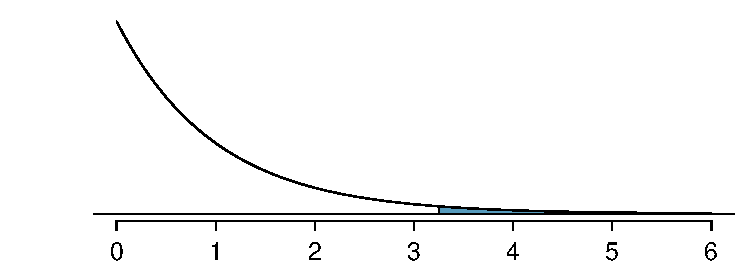
\includegraphics[width=0.65\textwidth]{ch_inference_for_means_oi_biostat/figures/fDist2And592/fDist2And592Shaded}
	\caption{An $F$ distribution with $df_1=2$ and $df_2=592$. The tail area greater than $F = 3.23$ is shaded.}
	\label{fDist2And592Shaded}
\end{figure}

The larger the observed variability in the sample means ($MSG$) relative to the within-group variability ($MSE$), the larger $F$ will be. Larger values of $F$ represent stronger evidence against the null hypothesis. The upper tail of the distribution is used to compute a $p$-value, which is typically done using statistical software.

\begin{example}{The $p$-value corresponding to the test statistic is equal to about 0.04. Does this provide strong evidence against the null hypothesis at significance level $\alpha = 0.05$?
}

The $p$-value is smaller than 0.05, indicating the evidence is strong enough to reject the null hypothesis at a significance level of 0.05. The data suggest that average change in strength in the non-dominant arm varies by participant genotype.	
	
\end{example}

\begin{termBox}{\tBoxTitle{The $F$ statistic and the $F$ test}
		Analysis of variance (ANOVA) is used to test whether the mean outcome differs across 2 or more groups. ANOVA uses a test statistic $F$, which represents a standardized ratio of variability in the sample means relative to the variability within the groups. If $H_0$ is true and the model assumptions are satisfied, the statistic $F$ follows an $F$ distribution with parameters $df_{1}=k-1$ and $df_{2}=n-k$. The upper tail of the $F$ distribution is used to represent the $p$-value.}
\end{termBox}

\subsection{Reading an ANOVA table from software}

The calculations required to perform an ANOVA by hand are tedious and prone to human error. Instead, it is common to use statistical software to calculate the $F$ statistic and $p$ value. The results of an ANOVA can be summarized in a table similar to that of a regression summary, which will be discussed in \MultipleRegressionChapter{Chapters~\ref{linRegrForTwoVar} and~\ref{MultipleLinearRegression}}{Chapter~\ref{linRegrForTwoVar}}.

Table~\ref{anovaSummaryTableForFamuss} shows an ANOVA summary to test whether the mean change in non-dominant arm strength varies by genotype. Many of these values should look familiar; in particular, the $F$ test statistic and p-value can be retrieved from the last columns.

\begin{table}[ht]
	\centering
	\begin{tabular}{lrrrrr}
		\hline
		& Df & Sum Sq & Mean Sq & F value & Pr($>$F) \\ 
		\hline
		famuss\$actn3.r577x & 2 & 7043 & 3522 & 3.231 & 0.0402 \\ 
		Residuals & 592 & 645293 & 1090 &  &  \\    \hline
	\end{tabular}
	\caption{ANOVA summary for testing whether the mean change in non-dominant arm strength varies by genotype at the \texttt{actn3.r577x} location on the ACTN3 gene.}
	\label{anovaSummaryTableForFamuss}
\end{table}

%JV: commenting this out for now because I don't think normal probability plots were introduced earlier as a method for checking normality.


\subsection{Multiple comparisons and controlling Type~1 Error rate}
\label{multipleComparisonsAndControllingTheType1ErrorRate}

\index{significance level!multiple comparisons|(}

Rejecting the null hypothesis in an ANOVA analysis only allows for a conclusion that there is evidence for a difference in group means. In order to identify the groups with different means, it is necessary to perform further testing. For example, in the \data{famuss} analysis, there are three comparisons to make: \resp{CC} to \resp{CT}, \resp{CC} to \resp{TT}, and \resp{CT} to \resp{TT}. While these comparisons can be made using two sample $t$-tests, it is important to control the Type I error rate. One of the simplest ways to reduce the overall probability of identifying a significant difference just by chance in a multiple comparisons setting is to use the Bonferroni correction procedure.

\begin{termBox}{\tBoxTitle{Multiple testing and the Bonferroni correction procedure}
		The scenario of testing many pairs of groups is called \term{multiple comparisons}. The \term{Bonferroni correction} suggests that a more stringent significance level is more appropriate for these tests:
		\begin{align*}
		\alpha^* = \alpha / K
		\end{align*}
		where $K$ is the number of comparisons being considered (formally or informally). If there are $k$ groups, then usually all possible pairs are compared and $K=\frac{k(k-1)}{2}$. In the test statistic $t$, use the pooled estimate of the standard deviation between groups, which is equivalent to $\sqrt{MSE}$. When calculating the $p$-value, use the $t$-statistic associated with $df_2$.}
\end{termBox}

\begin{example}{In the \data{famuss} dataset, there was strong evidence of differences in the mean strength change in the non-dominant arm between the three genotypes. Complete the three possible pairwise comparisons using the Bonferroni correction and report any differences.}

Use a modified significance level of $\alpha^* = 0.05/3 = 0.0167$. The pooled estimate of the standard deviation is $\sqrt{MSE} = \sqrt{1090.02} = 33.02$.

Genotype \resp{CC} versus Genotype \resp{CT}: 

\[
t = \frac{\overline{x}_1 - \overline{x}_2}{s_{\text{pooled}}\sqrt{\frac{1}{n_1} + \frac{1}{n_2}}} 
 = \dfrac{48.89 - 53.25}{33.02 \sqrt{\frac{1}{173} + \frac{1}{261}}} = -1.35\]
 
This results in a $p$-value of 0.18 on $df =592$. This $p$-value is larger than $\alpha^* = 0.0167$, so there is not evidence of a difference in the means of genotypes \resp{CC} and \resp{CT}.

Genotype \resp{CC} versus Genotype \resp{TT}: 
 
 \[
 t = \frac{\overline{x}_1 - \overline{x}_2}{s_{\text{pooled}}\sqrt{\frac{1}{n_1} + \frac{1}{n_2}}}
 = \dfrac{48.89 - 58.08}{33.02 \sqrt{\frac{1}{173} + \frac{1}{161}}} = -2.54\]

This results in a $p$-value of 0.011 on $df =592$. This $p$-value is smaller than $\alpha^* = 0.0167$, so there is evidence of a difference in the means of genotypes \resp{CC} and \resp{TT}.
 
Genotype \resp{CT} versus Genotype \resp{TT}:  
 
 \[
 t = \frac{\overline{x}_1 - \overline{x}_2}{s_{\text{pooled}}\sqrt{\frac{1}{n_1} + \frac{1}{n_2}}}
 = \dfrac{53.25 - 58.08}{33.02 \sqrt{\frac{1}{261} + \frac{1}{161}}} = -1.46\]

This results in a $p$-value of 0.145 on $df =592$. This $p$-value is larger than $\alpha^* = 0.0167$, so there is not evidence of a difference in the means of genotypes \resp{CT} and \resp{TT}.

In summary, the mean percent strength change in the non-dominant arm for genotype \resp{CT} individuals is not statistically distinguishable from those of genotype \resp{CC} and \resp{TT} individuals. However, there is evidence that individuals of genotype \resp{CC} and \resp{TT} are different. 
	
\end{example}

\textit{JV: add an example of situation in which ANOVA rejects, but no significant pairwise difference found}

\begin{caution}
	{Sometimes an ANOVA will reject the null but no groups will have statistically significant differences}
	{It is possible to reject the null hypothesis using ANOVA and then to not subsequently identify differences in the pairwise comparisons. However, \emph{this does not invalidate the ANOVA conclusion}. It only means we have not been able to successfully identify which groups differ in their means.}
\end{caution}


\index{significance level!multiple comparisons|)}

\index{analysis of variance (ANOVA)|)}

\section{Notes}



The material in this chapter is particularly important.  For many applications, $t$-tests and Analysis of Variance (ANOVA) are an essential part of the core of statistics in medicine and the life sciences.  The comparison of two or more groups is often the aim primary aim of experiments both in the laboratory and in studies with human subjects. More generally, the interpretation of tests and the conclusions that can are supported by tests illustrated in this chapter are used throughout the rest of the text and, indeed, in much of statistics.  

While it is important to master the details of the techniques of testing for differences in two or more groups, it is important not to lose sight of the important principles behind the tests.  A statistically significant differences between groups of the means of a response variables do not necessarily imply that group membership is the reason for the association.  Confounders may give a better explanation of observed differences.  A significant association does not necessarily imply causation, even if it is highly significant.  In most cases, causation can only be inferred in controlled experiments when interventions have been assigned randomly.   Students often find the distinction between paired and independent group comparisons confusing.  A careful reading of the problem is the only reliable method for picking the right approach.  Whenever possible, well-tested software should be used to compute test statistics and $p$-values. The \textsf{R} companion to this text supplements the conceptual approach emphasized here. 

Some details may benefit from further explanation.  It is generally prudent to use the form of the $t$-test that does not assume equal standard deviations, but the power calculations described in Section~\ref{ForDifferenceOfTwoMeans} are assume models with equal standard deviations.  The formulas are simpler when standard deviations are equal, and software is more widely available for that case.  The differences in sample sizes are usually minor and less important than assumptions about target differences or the values of the standard deviations.  If the standard deviations are expected to be very different more specialized software for computing sample size and power should be used. The analysis done after the study has been completed should use the $t$-test with unequal standard deviations.

Tests for significant differences are sometimes overused in science, with not enough attention paid to estimates and confidence intervals.  Confidence intervals for the difference of two population means show a range of underlying differences in means consistent with the data and often lead to insights not possible with the just the test statistic and $p$-value.  Wide confidence intervals may show that a non-significant test is the result of too much variability in the test statistic, perhaps caused by a sample size that was too small.  Conversely, a highly significant $p$-value may be the result of such a large sample size that the observed differences are not scientifically meaningful.  That may be evident in confidence intervals with very narrow width.

Finally, the formula used to calculate degrees of freedom $\nu$ for the Welch test is 

\[\nu = \dfrac{\left[(s_1^2/n_1) + (s_2^2/n_2)\right]^2}{\left[(s_1^2/n_1)^2/(n_1 - 1) + (s_2^2/n_2)^2/(n_2 - 1)\right]}\],
where $n_1, s_1$ are the sample size and standard deviation for the first sample, and $n_2, s_2$ are the corresponding values for the second sample.
Since $\nu$ is routinely provided in the output from statistical software, there is rarely any need to calculate it by hand.  The approximate formula $\text{df} = \min(n_1 - 1, n_2 - 1)$ always produces a smaller value for degrees of freedom and hence a larger p-value.

